\chapter{Adversarial attacks on federated learning networks
for medical image analysis}
\label{Bookchapter}

\begin{abstract}
\dropcap{F}ederated learning (FL) can significantly mitigate privacy concerns for Medical image analysis (MIA) systems. However, its decentralized and collaborative nature can bring new attack surfaces which might impose severe threats for participating clients.  
This paper investigates adversarial attacks where the adversary tries to fool other clients with manipulated data. 
% We presume a differentially private setting where the adversary has no access to other clients' models and data.
We investigate the credibility of known threat factors in a federated environment and discuss their importance. We demonstrate that domain-specific settings can lead to higher attacker success on MRI tumor and pathology imaging datasets.
In addition, we propose a scenario in which the adversary leverages the federated environment to devise a more powerful attack. We show that using gradient information from previous global model updates enables single-step attacks (e.g., FGSM) to outperform computationally expensive iterative methods so that the adversary reaches the same success rate $20 to 30$ times faster.



\end{abstract}

\blfootnote{This chapter is partly based on \faFileTextO~\emph{M. Beller. Toward an
    Empirical Theory of Feedback-Driven Development, ICSE'18 (Student Res
    earch Competition)}~\cite{BellerSRC2018}.
}


\newpage

% \dropcap{T}his is a introductory page.



% keywords can be removed
% \keywords{Federated learning \and Privacy-preserving machine learning \and  Medical imaging}


% \section{Introduction}

\section{Introduction}
\IEEEPARstart{I}n the past few years, federated learning (FL) has emerged as one of the mainstream machine learning (ML) paradigms and gained much attention in the field of medical image analysis (MIA). Federated learning enables hospitals and other healthcare providers to train machine learning models jointly with other hospitals without sharing sensitive data. It is applied to a wide scope of MIA tasks, successfully addressing data governance concerns. Notable works include brain tumor classification and segmentation, breast density classification, and covid-19 detection. \cite{sheller2020federated,dayan2021federated,rieke2020future}.



Although FL has mitigated many risks and concerns about multi-institutional collaborations, it is still vulnerable to other privacy issues. Several emerging attacks are proven to threaten FL networks. Adversarial clients might be able to change the model's prediction or gain information about other clients by actively changing its own model parameters or synthesizing fake input data.





This paper analyzes a group of attack scenarios called 'adversarial attacks.' A malicious client aims to cheat the model by adding subtle noise to its examples. The noise is so minimal that the change in the image is imperceptible for a human observer. However, it can cause the model to misclassify it. 
Adversarial attacks are the main source of vulnerability to the deployed FL models \cite{bouacida2021vulnerabilities,lyu2020threats,costa2021covert,lyu2020privacy}\. and are designed to fool the models that  are already trained 
% So their threat for the deployment phase 
passed their test phase and delivered for clinical use. 
% \\Although there is some research in the past in FL and MI, we believe that adversarial attacks could also be explored since they could be a threat to clinical decision-making.
% \\The attacks are analyzed in a federated setting to investigate their inter-client transferability.
\\We leverage the FL environment to propose a stronger attack and show that it enables adversarial clients to manipulate other benign clients to a high degree.  
We also show that proposed defense methods such as differential privacy still have limited effect against this attack.
In the following sections, we introduce adversarial attacks, sources of vulnerability, and our method.

\begin{figure}[t!]
 \centering
 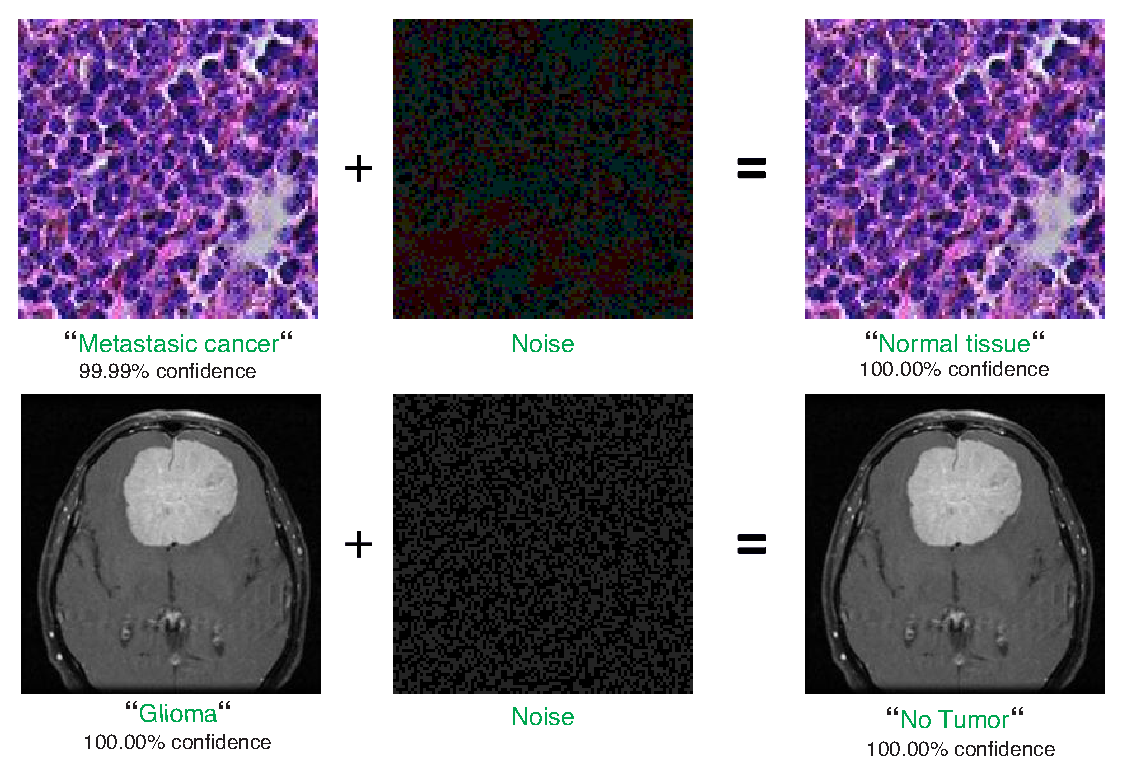
\includegraphics[width=0.52\textwidth]{Whatisads.eps}
 \caption{A schema of adversarial attacks to cancer detection systems}
 \label{fig:pgd-atta-comparison}
\end{figure}
 
 

%  Even if in indirect use and as a backbone for imaging software.
 \subsection{ Adversarial attacks }
Adversarial attacks are attributed to the linear characteristics of high-dimensional data. \cite{goodfellow2014explaining}. The crafted noise examples produced using one model might be able to manipulate other models. In FL setting, these attacks are also known as evasion attacks.\cite{biggio2013evasion,costa2021covert,ayub2020model,bouacida2021vulnerabilities}, are defined as if a malicious client tries to manipulate other clients with fake data.\\
At the same time, research on defense methods is also ongoing. Some studies tried to incorporate differential privacy (DP) as a protection measure in FL setting. Differential privacy was initially proposed to protect against privacy attacks, but it has also been applied against adversarial attacks.\cite{bouacida2021vulnerabilities,asgari2018vulnerability,wu2020evaluation}. Despite the ongoing research, there is no universal defense method against them.

We have introduced adversarial attacks in the scope of FL and MIA systems. We argue that distinct features of FL environments and MI make their combination highly vulnerable to adversarial attacks. \cite{chen2017targeted,chen2019deepinspect,ji2018model}.  The following paragraphs argue how each FL and MI expose new attack surfaces.
\\\textbf{Federated learning and adversarial attacks:} FL characteristics are known to elevate the impact of attacks known in the centralized setting. \cite{goldblum2020dataset,liu2022threats} The unique vulnerabilities of FL can be :
% We think the adversarial attacks on federated learning medical systems are notable important for three reasons, and this topic might not be explored properly. 
\begin{enumerate}[(i)]

\item{\textit{More data:} }
Each model received in every round has updated information about other clients. Adversaries can exploit this information to prepare stronger attacks.\cite{sun2019can,fang2020local,wang2020attack,song2020analyzing}
\item \textit{Open training:} In FL, the training process involves a lot of participants. Among them, one adversary could act maliciously.
\item{\textit{Standardized data pipelines:}} FAIR data stations and data standardization steps are inherent in many of FL networks in hospitals\cite{wilkinson2016fair}, near Global 
Electronic data management and medical communications (DICOM) integrated into the federated pipelines.
\cite{van2022ai}. Clients with more similar data are prone to attacks. \cite{miotto2016deep}
\item \textit{Scale of deployments:} FL networks have been deployed on a large scale in healthcare. Models act as a backbone of multiple inference software. FL networks in the deployment stage are especially weak against adversarial attacks. \cite{costa2021covert,bouacida2021vulnerabilities}.

\end{enumerate}
\textbf{Medical images and adversarial attacks}: Also, medical images have distinct features which makes the networks trained on them more vulnerable.
\begin{enumerate}[(i)]
    \item {\textit{Feature representation:}} Due to the inherent feature space of medical images, MIA systems are more vulnerable to this sort of attack than natural images. As shown in  previously published work, medical images have a narrower high-dimensional feature representation of images than natural images, causing trained networks to be over-parameterized. \cite{ma2021understanding} Over-parameterized networks are inherently easier to fool. \cite{Ye_2019_ICCV} As a result, medical imaging classifiers are easier to fool than natural image classifiers.  \cite{ma2021understanding} Several works have confirmed this by arbitrarily manipulating Funduscupy, Chest X-Ray and Dermoscopy data resulting in ... \cite{finlayson2019adversarial}. 
    \item \textit{Unique texture:}Medical images have limited texture diversity, and small texture perturbation in medical images can confuse classifiers to a high degree. \cite{ma2021understanding} This feature can be of advantage to the adversary's attacks, because they can perturb the texture in irrelevant areas and fool the classifier without manipulating the more important parts, e.g., the tumor area.\cite{ma2021understanding}. Which has, for example, been shown to effectively confuse tumor detection classifiers  \cite{gupta2022vulnerability}
    
\end{enumerate}



\subsection{Transferability factors}
Despite defense not always being an option, DL systems might be able to gain insight into their points of vulnerability. Some parameters and deployment settings might increase the chances of a successful attack.\\
Gaining such perception can be directly imported in security analysis so that the technicians know where the highest threat can be from, and they do not require a brute-force simulation of all the scenarios and parameter values, which is practically hard and in most cases impossible. 
\\The research is ongoing on attack transferability.\cite{gao2022boosting,elaalami2022bod,dai2021fast,duan2022novel,du2020hybrid,zheng2020efficient,shafahi2019adversarial,qiu2022framework}. In the MIA domain, transferability analysis has been done in a centralized ML setting, and the results are found to be domain specific. Factors such as data disparity, perturbation degree, and pre-training are shown to be crucial in attack transferability. However, their extent and optimal values might vary to a large extent. This difference can be attributed to the characteristics of the target imaging domain, texture of images, and whether the attack is white-box or black-box.\cite{ma2021understanding} \cite{bortsova2021adversarial}. \\ In an FL setup with a higher level of complexity, their findings might have limited pertinence. \cite{costa2021covert} One research question could be how FL can bring up new factors, and whether its optimal attack settings are concordant with the existing literature obtained from centralized data experiments. 
In this project we investigated potential factors in this setup, and discuss their effect on transferability.




\\\subsection{Our attack}

The adversarial client participating in an FL setup has access to previous model updates. We investigate a scenario where the adversary can enhance its attack using the gradient information from those model updates. However, obtaining gradient information might be a challenge, and also transferring them to the subsequent models causes drastic parameter change.\cite{zheng2020efficient}
We introduce an intermediary noise tensor we call \textit{Cross-round noise (CRN)} which utilizes previously received global model updates to generate noise and passes them to the next FL round. To initialize the next round and avoid parameter change, we regularize $L_{2}$ each noise channel by its mean value. 
\\This way can achieve better performance and improve transferability, with a much lower computation burden than the standard attack methods. %This can boost the computationally expensive attack models and bring higher capability.

% We assumed that the attacker doesn't necessarily have knowledge about model weights or inner settings of the target model, or the softwares that are build upon the model.\\




% \hl{

% Adversarial attacks are important in MEDICAL IMAGING  FL and not other attacks
% }

% \hl{tozieh bede ke chera evasion attack ro entekhab kardi va rabtesh be medical chie (masala model poisinning ya free rider chera na)}


% There are other manipulations but we chose adversarial attacks.
% 1- they preserver content
% 2- they designed for fool end-users and deployment.

% Like there are several attacks that can 
% causes the model not to converge or fail. 
% Other types of manipulations exist in the literature. Adversarial attaks are important for some reaasons, first, they aim presesrve the content of the image and the attack is imperceptible by human.% FL are more vulnerable during test phase.Mostly because a test phase before development can reveal impaired mod
%  In the medical imaging context, the deployment phase attacks are designed to manipulate the end-users, rather than hampering the training process. Adversarial attacks are only designed for the deployment phase, and are the only verified source of vulnerability of deployed FL models.el.
% Although but adverIt can impact clinical decision making. 
% the attacks during deployment phase % various reasons. Failure of models, communication bottlenecks, dropout of clients, non-robust aggregation, and poisoned model updates. 

% % Federated networks can be attacked during development or deployment phase. Here we focus on 
% Adversarial attack aim the end-users, \cite{ Vulnerabilities in FL}  after the model has passed its test phase. In the clinical setting, these manipulation to a federated network that could have directly impact the clinical desicion making.  Other forms of manipulations to FL exist. As an example failure of models, communication bottlenecks, dropout of clients, non-robust aggregation, and poisoned model updates can hamper the training proces



\\
\subsection{Organization of paper}


This paper evaluates the effect and degree of adversarial attacks on DP-enabled FL networks in MIA. To our knowledge, this is the first time malicious attacks are analyzed in federated MIA networks. We performed the most common attacks, namely PGD, basic iterative, and FGSM methods. Adversarial attacks are an essential threat to deep learning networks and significantly decrease performance. This is especially important in the MIA, where FL-trained networks are deployed as a tool to diagnose and analyze. We also assumed that some parameters might be essential to determine how transferable the attacks are, namely, the degree of perturbation and iteration steps. Which is not fully explored yet. We think that these parameters are vital since they balance the compromise between the imperceptibility of the noise and the success of the attack.\\ The study is done to detect cancerous images, namely GLioma, Meningioma, and histopathology. Tumor type classification is a multi-class classification of tumors in a setting with three participating hospitals. We did it with SOTA deep learning modes and discussed the importance of each potential factor in a DP-enabled environment. And discuss the provided model of attack.
%To the best of our knowledge, no study has investigated the scenarios for MIA.



We can summarize our contributions as follows.

\begin{itemize}
  \item To the best of our knowledge, this is the first study introducing and investigating adversarial attacks on FL in the MIA. We discuss its importance for the medical imaging society, potential real-world threats, and implemented attack scenarios.

\item We test and compare the popular attacking methods on a DP-enabled setting, where DP requirements are imposed on both sides of the communication. Although some studies have adversarial attacks in medical imaging, None has investigated them in a differentially private setting.

  \item  We introduce a new attack and show the superiority of our model compared to the popular models. We show that sometimes single-step calculation can outperform computationally expensive models.
%   \item We discuss how unexpolored parameters can play in this setting and affect the transferability, and perceptibility.
    \item We discuss how domain-specific parameters can affect the transferability ,and try to estimate their optimal values in our setting. We calculate attack success rate and error transfer rate in each medical imaging task.
  \item We do all of the above on popular MIA datasets and tasks, namely detecting and classifying cancer in brain MRI and histopathology images
  
\end{itemize}


The rest of paper is organized as follows, the next section discusses adversarial attacks on MIA and FL systems. Section \ref{sec:prelimianries} introduces FL, differential privacy and attack models,  \ref{sec:attack} introduces our attack method. Next section introduces our attack, results and then discussion and the last section will be conclusion.
% \\\hl{bishtar dalil mituni biari ke chera taeene levele noise mohemme wa chera in parametera ehtemalan moheman va bayad baresi beshan }
% \hl{\\ We study effect , number of participants, chera mohemme (ba literature sabet kon)}\\
% \hl{\faClockO  Adv attack Is not noise}\\
\section{Related work}
\label{sec:related}


The effect of adversarial attacks on MIA has been studied in several works. Modalities such as chest X-ray, MRI \cite{finlayson2019adversarial,bortsova2021adversarial,asgari2018vulnerability,ma2021understanding} and CT scan
\cite{navarro2021evaluating}
  segmentation and classification of medical images are vulnerable to adversarial attacks. \cite{ozbulak2019impact} classification \cite{asgari2018vulnerability}.
\\Several works worked to discover important parameters on attack transferability.
\cite{gao2022boosting,elaalami2022bod,dai2021fast,duan2022novel,du2020hybrid,zheng2020efficient,shafahi2019adversarial,qiu2022framework}. Gradients of different samples in one batch\cite{shafahi2019adversarial}, extent of data augmentation \cite{gao2022boosting}, variation in input gradients \cite{qiu2022framework} are shown to be important transferability. Zhang et al. analyized the impact of transfer learning on black-box attack.\cite{zhang2020two}. Another work \cite{zheng2020efficient} utilized the transferability of examples to enhacne  robustness, although their method was proposed for white-box setting. 

% The effectiveness of the above methods is not apparent in the federated setting.




In MIA,  perturbation degree
has been shown previously as a less explored but highly deterministic parameter in attack setting, and might need visual tuning.\cite{bortsova2021adversarial}. Optimal values of standard black-box\cite{bortsova2021adversarial}, and white-box \cite{ma2021understanding} are domain-specific. Also iteration steps $\alpha$, can be highly deterministic in centralized setting. \cite{tashiro2020diversity} \cite{cai2018curriculum}. 
% \textbf{Adversarial attacks on Federated learning} 
 
% \\Also, some enhancement methods have been proposed. 

 
Methods such to detect the attack
\cite{yin2021exploiting,drenkow2022attack,ma2021understanding }
or protect the models from adversaries\cite{lin2021certified,yuan2019adversarial,papernot2017practical,biggio2018wild,li2022review} are also discussed in ML domain.
 Adding noise to the exchanged model with clipping model updates is effective in several forms of adversarial attacks.\cite{bouacida2021vulnerabilities}. In norm-bound defense, the server enforces an upper-limit norm-bound. Several studies have investigated black-box PGD attacks in an FL environment with norm-bound situation. \cite{sun2019can,wang2020attack} . In the clinical setting,
% Some models have proposed differentially private settings.
\cite{shao2019stochastic} DP models are used in clinical EHR data\cite{li2019distributed}  \cite{ma2019privacy} and neuroimaging data \cite{li2020multi} in multi-site setting. 


However, other studies have shown that adversary can circumvent the detection if it is aware of it \cite{yin2022adc} , they function in very specific conditions,\cite{yin2022adc}  might have drastic parameter change\cite{zheng2020efficient},or they require too much computational power \cite{yuan2019adversarial,uesato2018adversarial,yin2022adc}. 


% and less evaluated in MIA domain.
% \\\hl{Yejuri in kosshere CVPR ro biar ke na sikh besuze na kabab}

% \\\hl{\faClockO bebin stucking ro mituni biari,Using knowledge from previous rounds / stacing:
% age na inaro biar:
% \\\faQuestion Effect of perturbation degree ro kia barresi kardan
% \\\faQuestion Effect of alpha ro kia barresi kardan
% }
% \\\hl{\faClockO Maqalati ke asare noise level be FL tajihan}\\
% \hl{\faClockO Maqalati sanjidan number of clients ro sanjidan}\\
% \hl{\faClockO Other attacks on MI has been done}\\
% \hl{\faClockO Some privacy attacks on FL MI has been done}



\section{Preliminaries}
\label{sec:prelimianries}
\subsection{Federated Learning}



Federated learning enables multiple data owners with private datasets to jointly train a global model based on local models. The  optimization problem could be formulated as
${w} = \sum\limits_{i=1}^{N}{p_{i}{w}_{i}}$ , ${w}_{i}=\arg\min\limits_{{w}_{i}}{\left(\mathcal{L}(\mathcal{D}_{i};{w})\right)}$ where $N$ is the number of data owners, $\mathcal{L}(\mathcal{D}_{i};{w})$ is a loss function indicating global model parameters  ${w}$ of local datasets.  
 The learning procedure is an iterative process containing local and global steps. Each data owner trains a global model on its local dataset received from a global server in local iterations. The global server aggregates the updated local models for the next round for updating the global model. 
 
 The global server selects a subset of clients at each global round and sends the most recent global model to them. Then each client performs local training over its dataset for a selected number of epochs. The updated local models are calculated on selected batches. Local optimization can be formulated as ${w}_i \leftarrow {w}-\eta\cdot \nabla \mathcal{L}({w};\mathcal{D}_{i})$, where 
%  $\beta$ is a batch randomly sampled from the local dataset and
 $\eta$ is the learning rate. Several local iterations might be required to go over all the local data. Local training procedures can be done for several local epochs.
%
(3) The global model can be updated based on the local models ${w}_i$ is shared for aggregation: 
${w} = \sum\limits_{i=1}^{N}{p_{i}{w}_{i}}$, to update the global model for the next FL round.

%-------------------------------------------------------------------------
\subsection{Differential Privacy}\label{sec:Differential Privacy}



 Differential privacy (DP) requires FL parties to ensure an attacker can not distinguish data records. For multi-party systems $\mathcal M: \mathcal{X}\rightarrow \mathcal{R}$ mapping from domain $\mathcal{X}$ to target domain $\mathcal{R}$, differential privacy  $(\epsilon, \delta)$-DP defines a measure to evaluate  performance of privacy preserving mechanisms.
For two adjacent datasets $\mathcal D_i, \mathcal D_i'$. DP introduces a bounding parameter $\epsilon > 0$ , represents the ratio of probabilities of two datasets bounded by performing the privacy preserving mechanism  $\delta$. It can be summarized by the following definition \cite{dwork2014algorithmic}:
 
\begin{definition}
Mapping $\mathcal M: \mathcal{X}\rightarrow \mathcal{R}$ is $(\epsilon, \delta)$-DP,
if for all measurable subsets of target domain $\mathcal S\subseteq \mathcal{R}$ and for any two adjacent datasets $\mathcal D_i, \mathcal D_i'\in \mathcal{X}$, 
\begin{equation}\label{equ:Differential privacy}
\emph{Pr}[\mathcal M(\mathcal D_i)\in \mathcal S]\leq e^{\epsilon}\emph{Pr}[\mathcal M(\mathcal D_i')\in \mathcal S]+\delta.
\end{equation}
\end{definition}
% As a guaranteed way to obtain $(\epsilon, \delta)$-DP, gaussian mechanism proposed in \cite{dwork2014algorithmic} can be used. 
In FL setting,  $(\epsilon, \delta)$-DP can be achieved by adding noise to the updated models.
% To ensure privacy for both global server and clients,
Global differential privacy is a privacy mechanism imposes a double-sided $(\epsilon, \delta)$-DP requirement for both uplink and downlink channels\cite{wei2020federated}.
From the uplink perspective, all clients $1\leq i\leq N$, clip their updates  $\Vert{w}_{i}\Vert \leq C$, where ${w}_{i}$ denotes the updates weights from the $i$-th client before perturbation and $C$ is the clipping threshold. To satisfy a $(\epsilon, \delta)$-DP requirement for the downlink channels, additional noise ${n}_{\text i}$ is   added by the server, so each client $i$ receives $\tilde{w_i}$ perturbed model\cite{wei2020federated}.

 
%  ing ${w}_{i}$. 
%  and ${w}$ are the aggregated parameters at the server to be broadcast to the clients.

%===========================================================================

% \subsection{Adversarial attacks}


\subsection{Adversarial attacks }

Introduced by \cite{szegedy2013intriguing}, adversarial examples are attributed to the linear characteristics of high-dimensional data. \cite{goodfellow2014explaining} Based on the threat model and goal and knowledge of the Adversary, the attacks can be categorized from different points of view.
\\\textbf{Adversary's goal} Adversarial attacks can be categorized based on the adversary's goal. \textit{Untargetted attacks} aim to reduce the model performance,  regardless of the class to which a test sample belongs. \textit{Targeted attacks} force the model to output certain labels.
\\\textbf{Adversary's knowledge} Based on the adversary's knowledge, attack can be  \textit{white-box},
meaning that the Adversary has complete knowledge about other clients' network architecture, gradients, and parameters. In such a setting, it can easily manipulate the model. The literature has extensively investigated them, and also their mathematics has been investigated.\cite{tramer2017ensemble} \cite{xu2020adversarial}. In \textit{black-box} heuristics, the Adversary doesn't have access to the surrogate model. In the black-box setting, however, it can interact with the model. They can feed inputs and receive outputs of the surrogate model. And improve the attack by observing the model outputs. Some black box might have limited knowledge about design of the surrogate model.\cite{yue2021black,9000972,cheng2019improving}

% attack can be \textit{black-box},  meaning that the adversary does not know about the model parameters or gradients of the victim network, but can interact with the model and query its output for given samples. adversary, has full knowledge about the victim network, including its layer weights and and parameters. White-box adversaries are the most powerful ones.



% \begin{figure}[t!]
%  \centering
% %  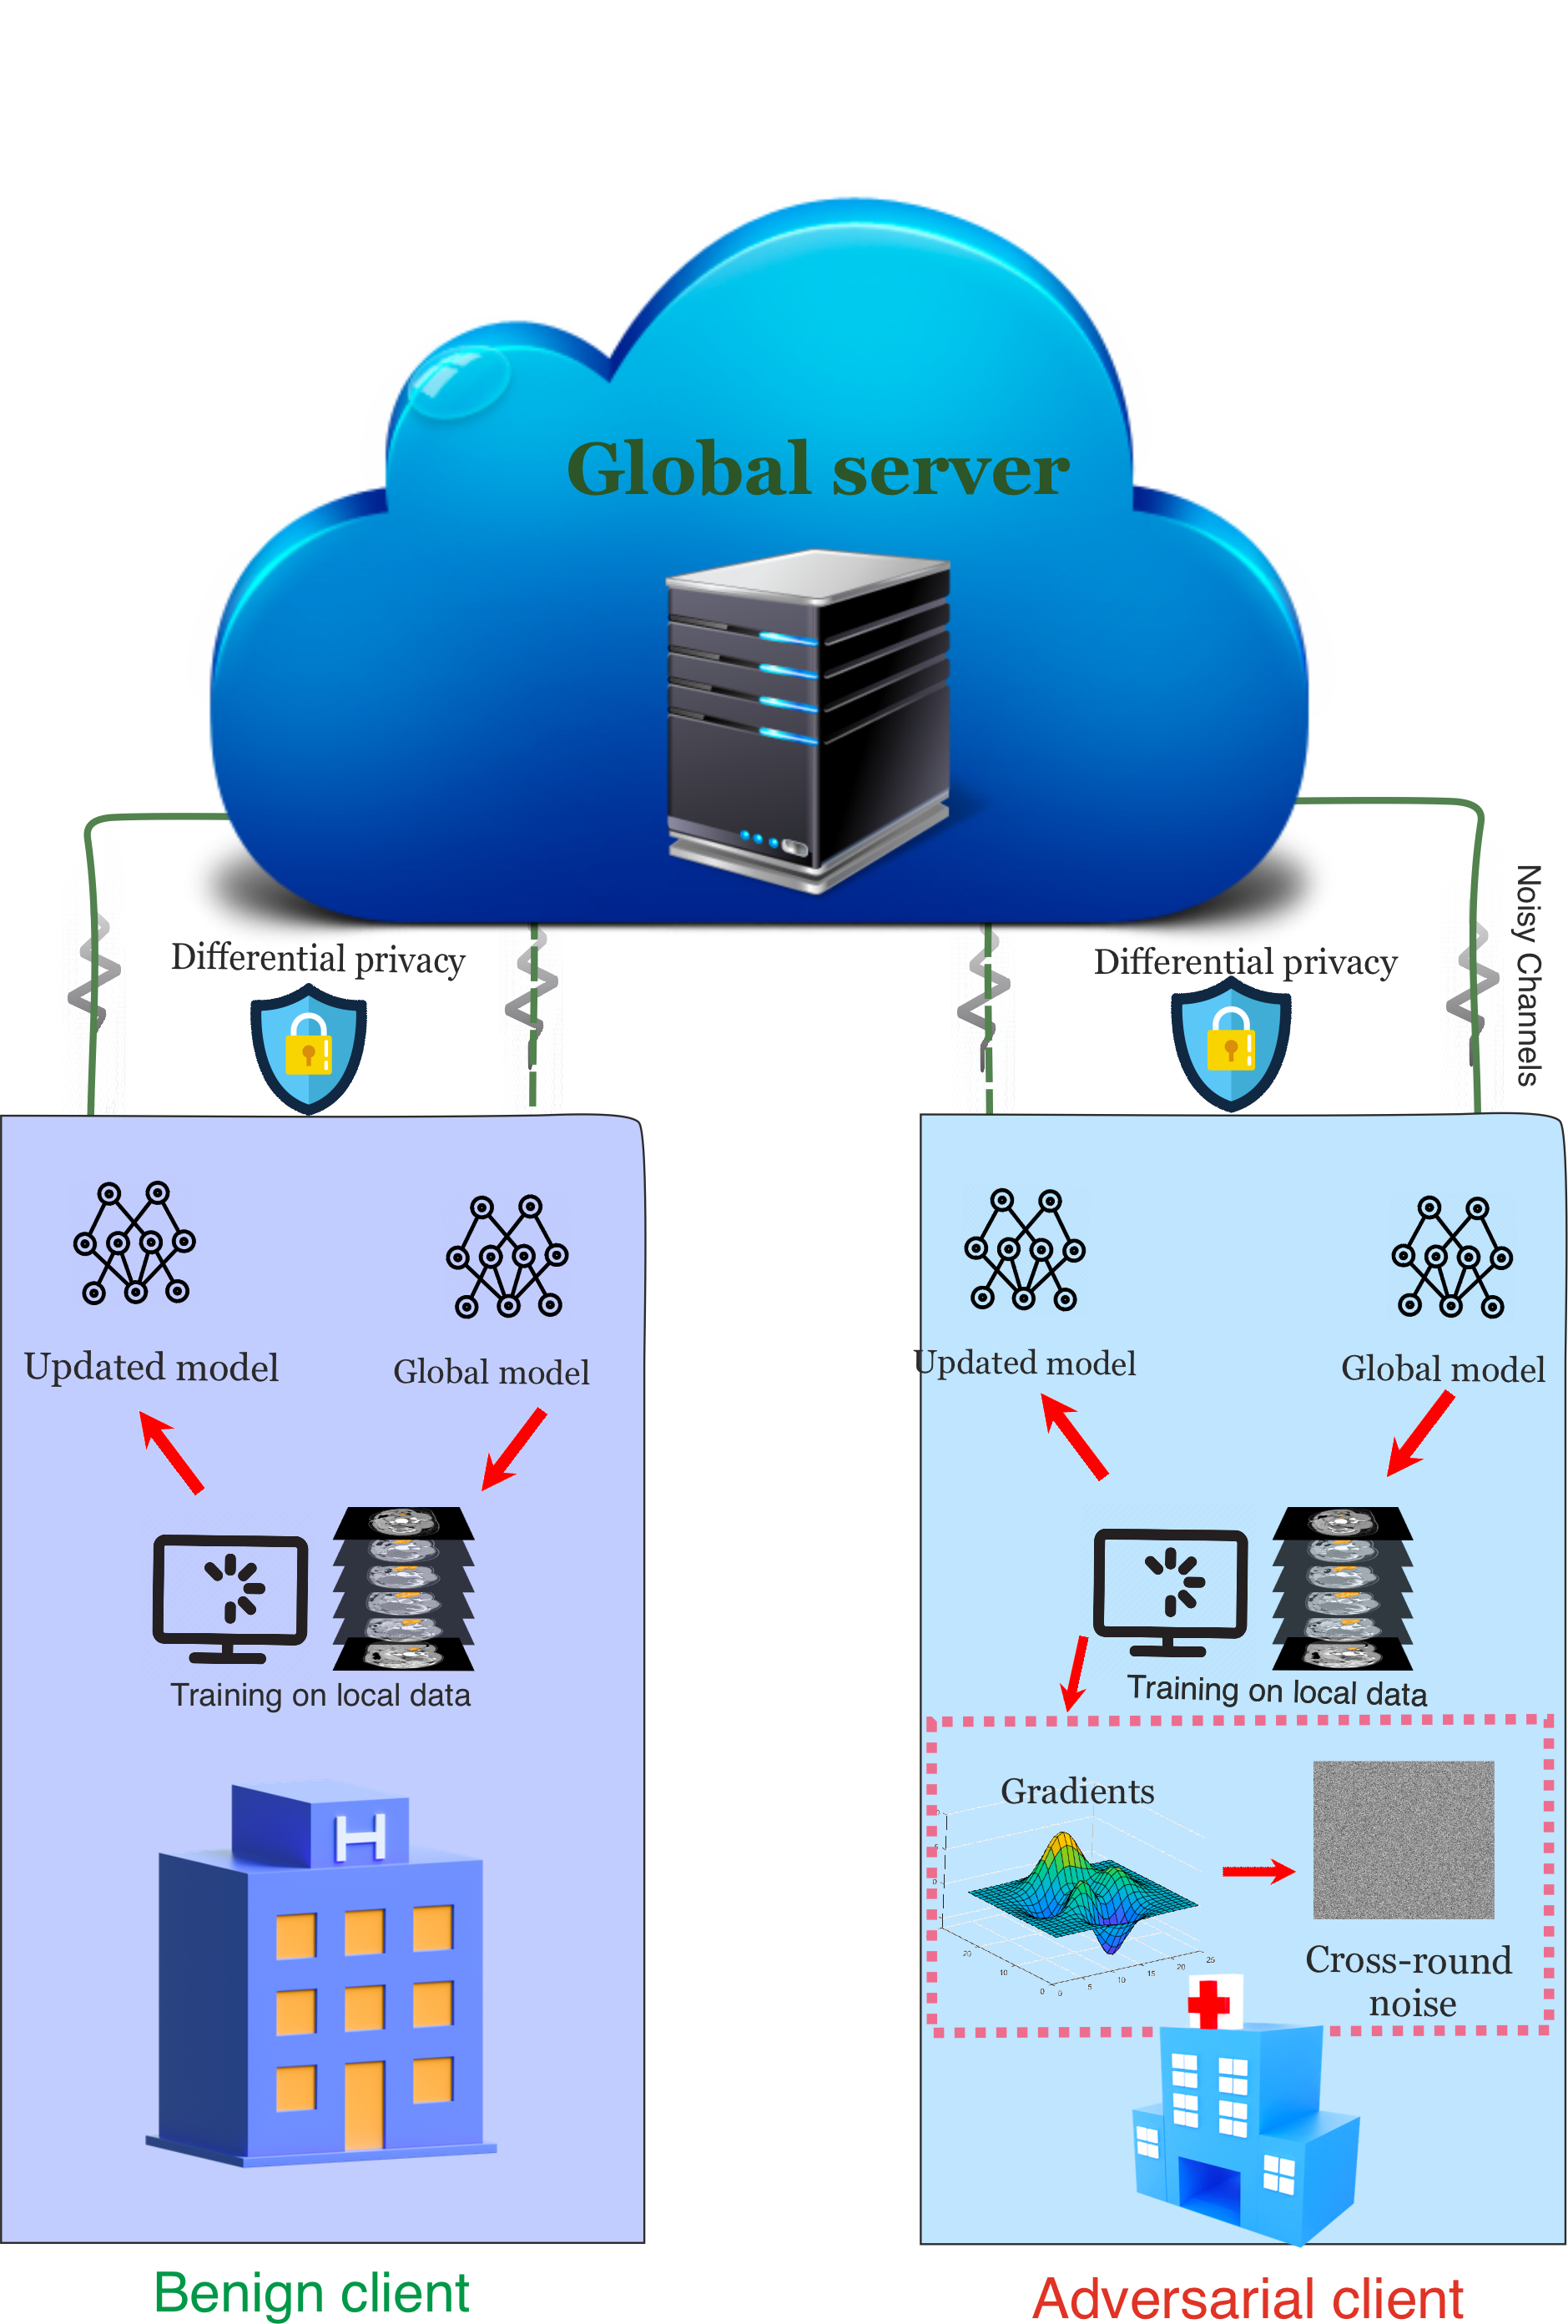
\includegraphics[width=0.50\textwidth]{Adversarialattacks.png}
%  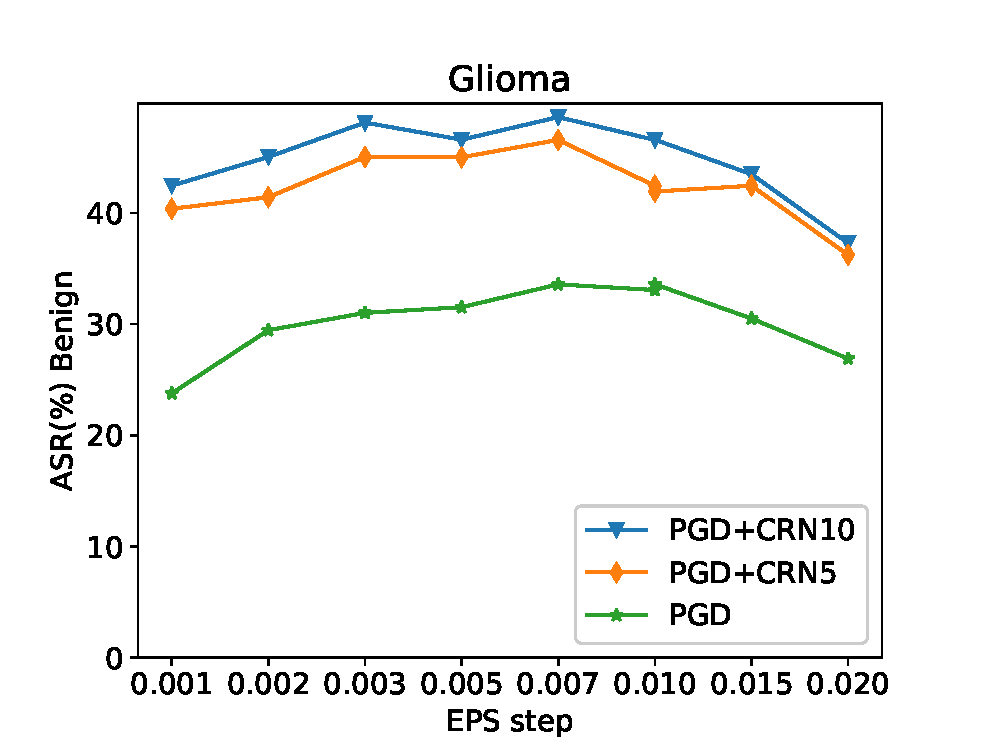
\includegraphics[width=0.50\textwidth]{Glioma_ASR_EPS_steps}
%  \caption{A schema of our method, at each FL round, the adversary transforms the gradients into cross-round noise, while acting as a benign client and not tampering the training process}
%  \label{fig:pgd-atta-comparison}
% \end{figure}


\begin{figure}[t!]
 \centering
 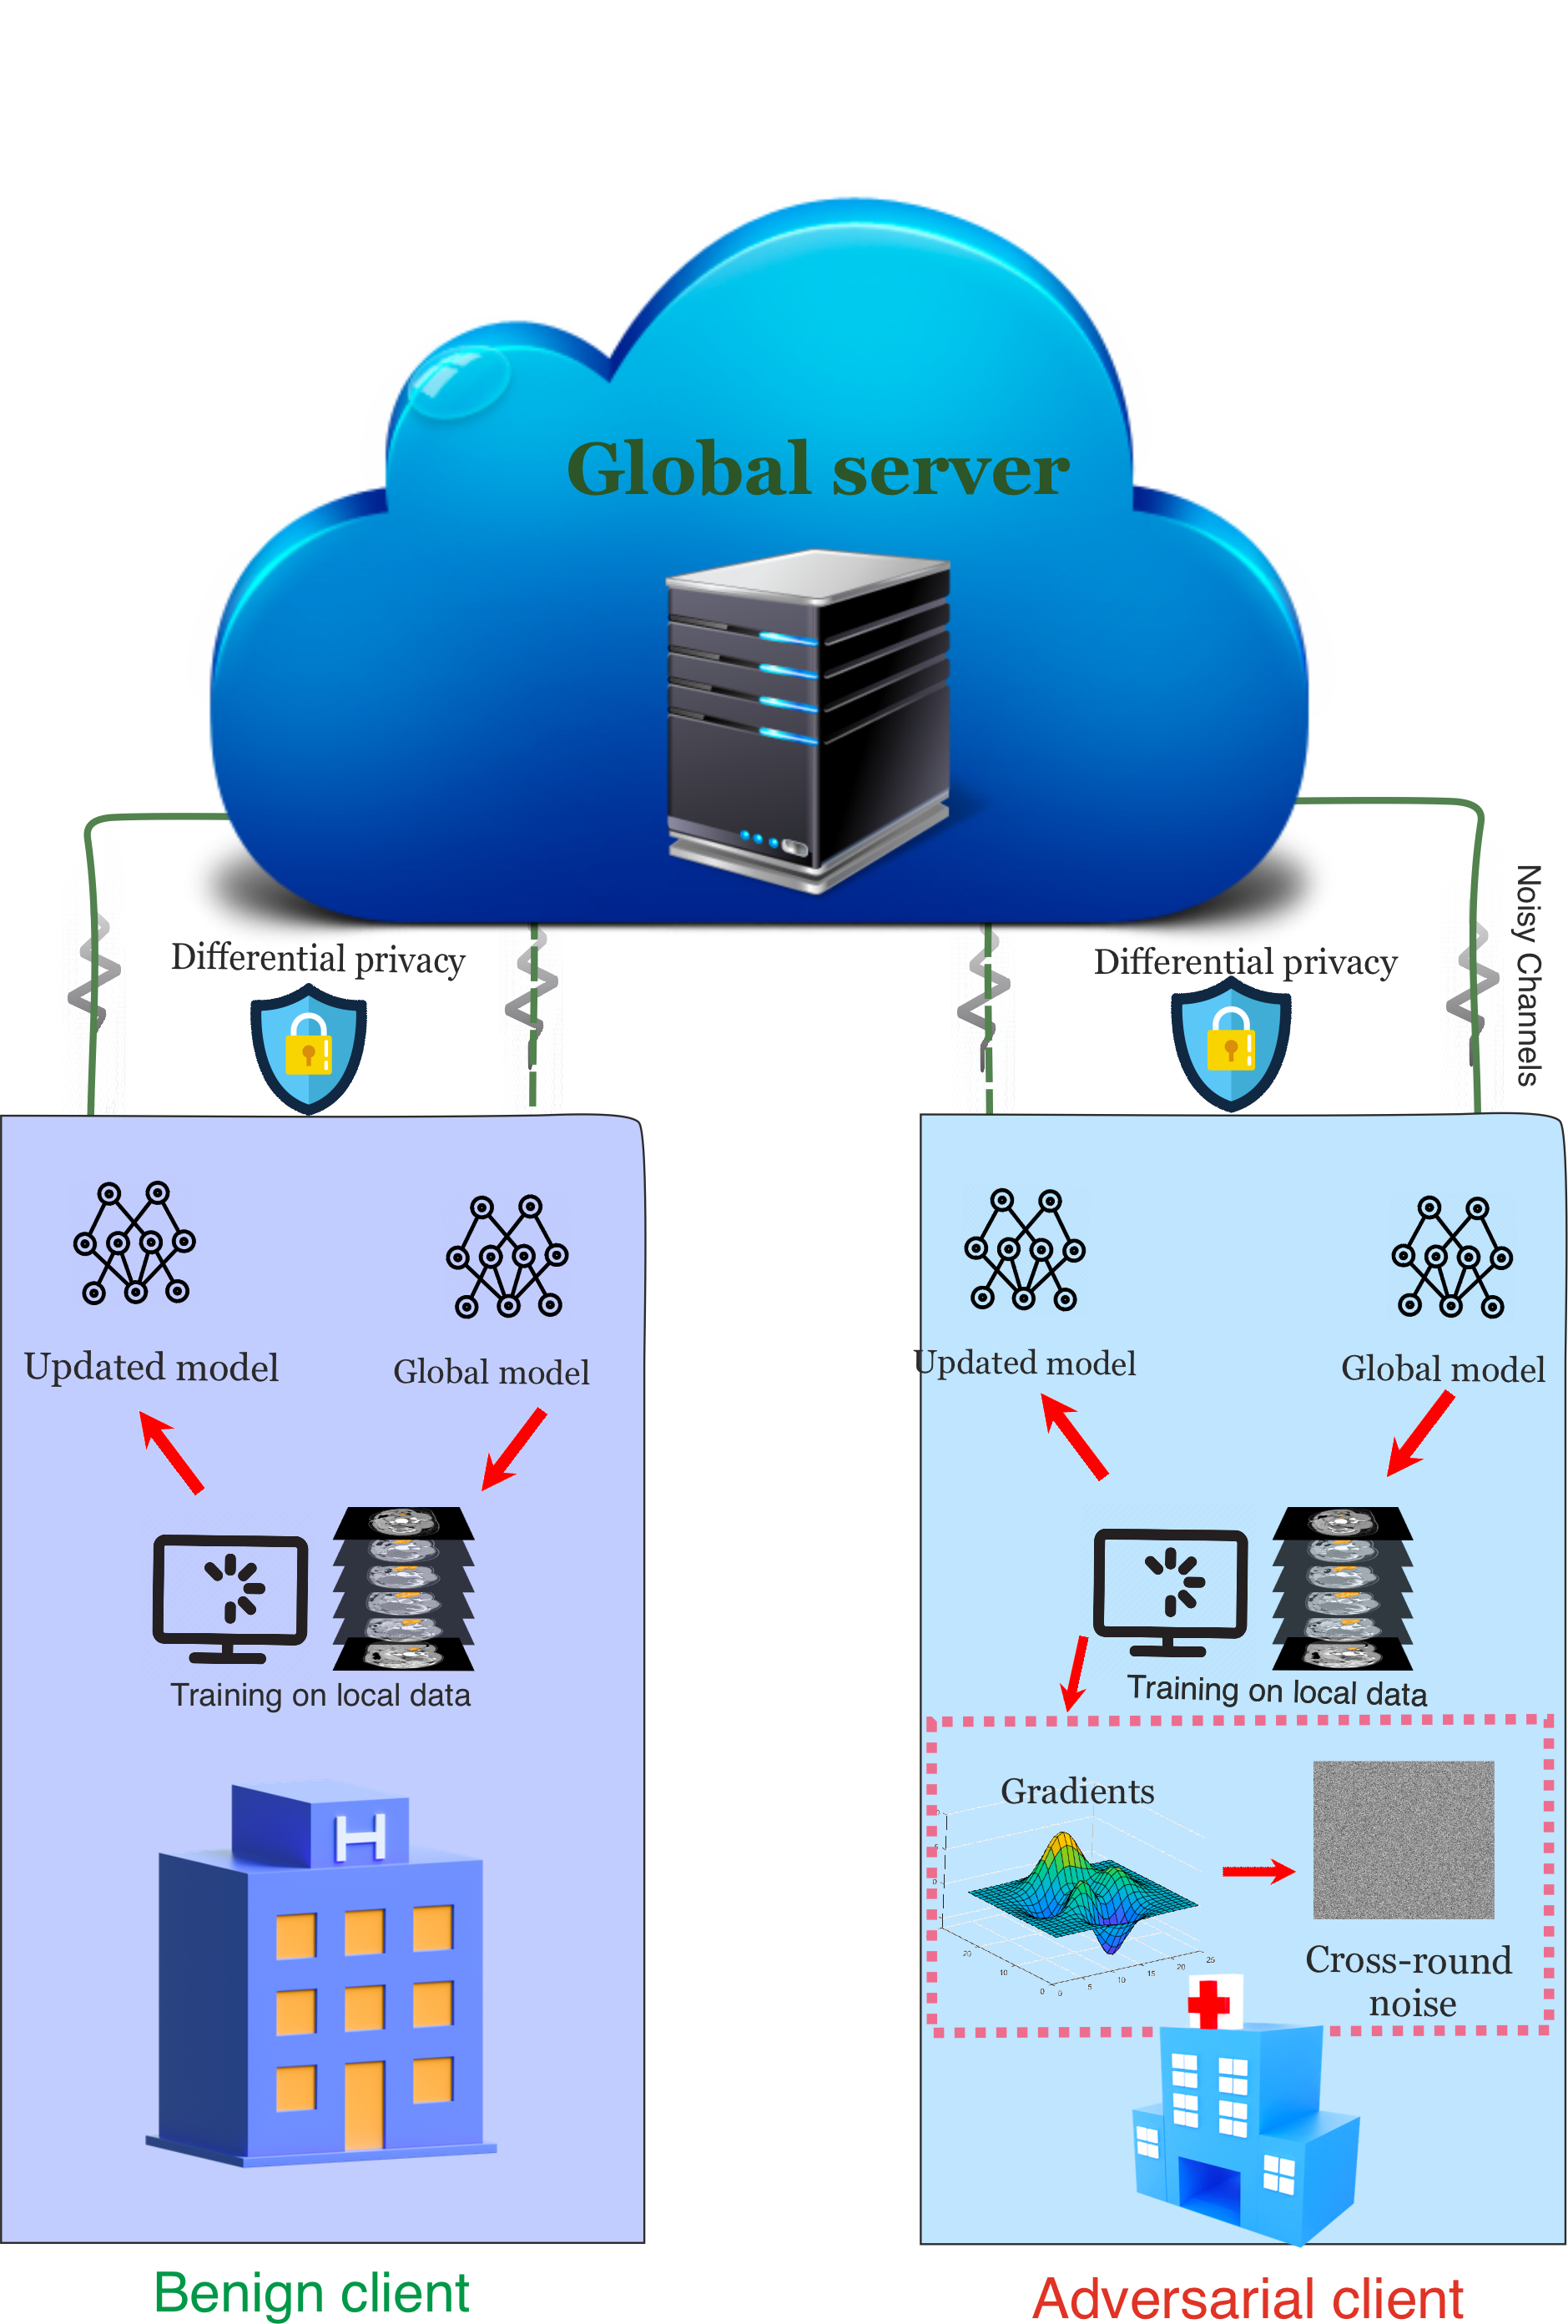
\includegraphics[width=0.50\textwidth]{Adversarialattacks.png}
 \caption{A schema of our method, at each FL round, the adversary transforms the gradients into cross-round noise, while acting as a benign client and not tampering the training process}
 \label{fig:pgd-atta-comparison}
\end{figure}

\subsection{Attack models}
Numerous adversarial attacks have been proposed by the literature in order to fool deep neural networks and produce false predictions. Adversarial attacks work through injecting a guided imperceptible noise that fools the trained deep learning model. Popular attack methods are Projected Gradient Descent (PGD), Fast Gradient Sign Method (FGSM, and Basic Iterative Method (BIM. Each will be discussed in this section.

\textbf{FGSM:} Fast Gradient Sign Method (FGSM) \cite{szegedy2013intriguing}is a fast yet effective method which produces adversary image with one step of calculation. Assuming input $x$ and its corresponding target $t$, FGSM calculates gradient of $x$ w.r.t the loss function ${\partial \mathcal{L}}/ \partial {x}$.

\begin{equation}
\label{eqt:fgsm}
    \bm{\hat{x}} = \bm{x} + \epsilon \cdot sgn\big(\nabla_{\bm{x}}{\mathcal{L}}(g(\bm{x};w)\big)
\end{equation}

where epsilon $\epsilon$ is a hyper-parameter which determines adversarial noise level. $g(\bm{x};\bm{w})$ is the output of neural network with respect to the input $x$ and parameter set $w$. $sgn(.)$ is the sign function. The result of sign function goes through a clipping function to impose a maximum bound in change to the perturbation $\epsilon \cdot sgn\big(\nabla_{\bm{x}}{\mathcal{L}}(g(\bm{x};\bm{w})\big)\in [-1,1]$.

\textbf{BIM:}  Basic Iterative Method (BIM) is an extension of the FGSM method, By Kurakin et al.\cite{kurakin2018adversarial} repeatedly do the process in FGSM, using a small step-size and $\bm{\hat{x}^{1}} = \bm{x}$. BIM is stronger than FGSM and requires smaller perturbations.

\textbf{PGD:} Madry et al. \cite{madry2017towards}proposed their own version of the BIM attack. In Projected Gradient Descent (PGD) \cite{madry2018towards}
the attack starts with a uniform random initialization. The update formula for PGD attack can be written as: 
\begin{equation}
\label{eqt:pgd}
    \bm{\hat{x}}^{t+1}=\Pi_{P_\epsilon(\bm{x})} \Big( \bm{\hat{x}}^t + \alpha \cdot sgn\big(\nabla_{\bm{x}}{\mathcal{L}}(g(\bm{\hat{x}}^t;\bm{w}),t)\big)\Big)
\end{equation}
Where $\bm{\hat{x}}^{k}$ is the perturbed data in $k$-th iteration, and $P_\epsilon(\bm{x})$ is the projected gradient descent function, which is done by first finding sign values, and then projecting the result to a small neighborhoud of the input ${x}$. This possible parameter spaces determines the set PGD attack samples that an adverdsary can use. PGD is one of the strongest attacks and is a universal first-order adversarial method. Technically, aside from formulazing the problem as projected gradient, PGD is similar to BIM but with random small initialization. We report results with PGD. With same number of iterations, BIM had the same results, or the difference was negligilbe.
	
% \subsection{Optional}
% blackbox/wihtebox
\section{Enhanced adversarial attack }
\label{sec:ourattack}
In this section we introduce our method to enhance the existing adversarial attacks in an FL setting.

\subsection{Threat model}


% \begin{algorithm}[th]
%  \caption{Adversarial Training with Transferable Adversarial Examples (ATTA)}\label{alg:atta}
%  \begin{algorithmic}[1]
%  \State \textbf{Input}: Padded training dataset $D_{nat}$, model $f_\theta$, attack algorithm $\mathcal{A}$, perturbation bound $\epsilon$, the number of epochs to reset perturbation $reset$
%  \State Initialize $\theta$
%  \State Initialize $D$ by cloning $D_{nat}$
%  \For{$epoch = 1 \cdots N$}
%  \For{$x_{nat},y$ in $D_{nat}$ and corresponding $x \in D$}
%  \If {$epoch\ \%\ reset\ =\ 0$}
%  \State $\beta \gets$ a small random perturbation
%  \State $x \gets x_{nat} + \beta$
%  \EndIf
%  \State Store the transformation $T_{aug}$ for the inverse augmentation:
%  \State $x_{aug}, x_{nat, aug}, T_{aug} \gets \dataaug(x, x_{adv})$
%  \State $x^* \gets \mathcal{A}(f_{\theta}, x_{nat, aug}, y, x_{aug}, \epsilon)$
%  \State $\theta \gets \theta - \nabla_{f_{\theta}} \frac{\partial \mathcal{L}(f_\theta, x^*, y)}{\partial \theta}$
%  \State $x \gets \inverseaug(x, x^*, T_{aug})$
%  \EndFor
%  \EndFor
%  \end{algorithmic}

% \end{algorithm}




We consider a scenario in which one FL participant is malicious or is controlled by a hostile adversary. The adversary tries to fool the global model by generating images similar to its real data.
We assume that the central server is honest and trusted.\\\textbf{Goal of adversary:}
The adversary's Goal is to manipulate the global model so that the global model has a higher classification error.  \\
\textbf{Knowledge of adversary:}
In a realistic scenario, the malicious party only can see its own data $D_{i}$, and knows the DNN architecture and the global model weights that it receives each round. \\
\textbf{Capability of adversary:}
No special privilege or Capability is assumed for the adversary. Similar to other clients, the adversary has control over its own training procedure and data, and it can not manipulate other clients' data or the general learning process. (e.g., local computations, communication with central server and aggregation process, DNN architecture, and optimization functions). It can interact with the model, query the outputs, and calculate the gradients. The adversary doesn't use the training data.




\subsection{Cross-round noise}



Adversarial examples being developed in the inference time, the adversary might not have the necessary computing power as they have during the training time. Also, sometimes inference is being done on third-party applications on edge devices where they don't have GPUs.
This might be crucial for the adversary, that it can prepare the attack samples with less computations. Iterative methods, such as PGD, require too much computational power to develop the examples. even more than normal training itself. \cite{zhang2019you} The problem could be worse for high-resolution or whole-slide images.
Also, PGD needs the target and surrogate to be highly similar to ensure transferability. However, models being noisy causes high inter-client variability, as a protection measure.

% Federetaed environemtn can introduce new surfaces to enhance adversarial transferability.  Gather more information about other clients by utilizing  global model upates.\cite{lyu2020threats}


% \begin{figure}[htbp!]
%  \centering
%  \includegraphics[width=0.10\textwidth]{Adversarial0attacks-7.eps}
%  \caption{Traditional adversarial training (PGD-$k$) (a) and ATTA-$k$ (b). $C$ is the connection function which improves the transferability between epochs.}
%  \label{fig:pgd-atta-comparison}
% \end{figure}
Incorporating prior knowledge already available from the global model, the attack can be initialized from a proper baseline so the computation might be reduced. Also, it might diminish the bias and lead to a broader estimation of other clients.



We introduce an intermediary noise tensor we call \textit{Cross-round noise} which extracts features from received global and is calculated alongside local epochs. The noise gets updated and passed to the next FL round. 
We use a function for the adversary to produce a noise based on ${L}_{2}$ regularized gradients at each FL training round. Then in the test phase, we use the noise to initialize the values for adversarial attack algorithms. 



\begin{algorithm}[t!]
\caption{Training procedure}
\label{alg:NbAFL}
\LinesNumbered
\KwData{$T$, $\beta$, ${w}^{(0)}$, $\mu$, $\epsilon$ and $\delta$}
{Initializing parameters: $t = 1$ and ${w}^{(0)}_{i} = {w}^{(0)}$ and ${{\mathcal{\delta}}^{(t)}=0}$} $\forall i,t$\\
\While {$t \le T$}
{
\textbf{Local training:}\\
\While {$\mathcal C_i\in \{\mathcal C_1, \mathcal C_2, \ldots,\mathcal C_{N}\}$}
{
Clients update their models ${w}^{(t)}_{i}$ as\\
% \quad\quad ${w}^{(t)}_{i}=\arg\min\limits_{{w}_{i}}{\left(F_{i}({w}_{i})+\frac{\mu}{2}\Vert {w}_{i}-
\quad${w}^{(t)}_{i}=\arg\min\limits_{{w}_{i}}{\left(\mathcal{L}_{i}({w}_{i})\right)}$\\
Clients clip parameters ${w}^{(t)}_{i} = {w}^{(t)}_{i}/\max\left(1,\frac{\Vert{w}^{(t)}_{i}\Vert}{C}\right)$\\
Clients add Gaussian noise\\ $\widetilde{{w}}^{(t)}_{i}={w}^{(t)}_{i}+{n}^{(t)}_{i}$\\
}
\textbf{Global update:}\\
Global server individual models ${w}^{(t)}$ as\\
\quad\quad ${w}^{(t)} = \sum\limits_{i=1}^{N}{p_{i}\widetilde{{w}}^{(t)}_{i}}$\\
Global server adds Gaussian noise \\
\quad\quad$\widetilde{{w}_{i}}^{(t)}={w}^{(t)}+{n}_{\text i}^{(t)}$\\
\If{$t \ge \beta$}
    {
% \textbf{Adversairal client:}\\
  \textbf{Adversarial client} $\mathcal C_{m},   \mathcal X \in \mathcal D_m:$
  % ,  {\mathcal{\delta}^{(\beta)}=0,$:}\\
% \quad\quad
\\Adversary performs gradient regularization \\
\quad{${{\nabla_{\mathcal{X}}\mathcal{\hat{L}}\gets \nabla_{\mathcal{X}}\mathcal{L}(\mathcal {\delta}^{(t-1)},\widetilde{{w}_{m}}^{(t)}})}$}\\
% ${\mathcal{\delta}}^{(t)}\gets \epsilon . sgn(\nabla_{\mathcal{X}}\mathcal{\hat{L}}(\mathcal {\delta}^{(t-1)},\mathcal{X},\widetilde{{w}_{m}}^{(t)})$
% \quad\quad${{\mathcal{\delta}}^{(t)}\gets \epsilon . sgn(\nabla_{\mathcal{X}}\mathcal{\hat{L}}(\mathcal {\delta}^{(t-1)},\widetilde{{w}_{m}}^{(t)}}))$
\\Adversary projects the gradient \\

\quad$\mathcal{\delta}^{(t)}\gets \Pi_{P_\epsilon(\bm{0})}(\nabla_{\mathcal{X}}\mathcal{\hat{L})}$
}
% Test the received parameters $\widetilde{\mathbf{w_{i}}}^{(t)}$ using local dataset\\
% 
\\$t\leftarrow t + 1$}
% #2ndPart#########################
% #2nd Part#########################
% #2nd Part#########################
% #2nd Part#########################
% #2nd Part#########################
% #2nd Part#########################
% #2nd Part#########################
% #2nd Part#########################
% #2nd Part#########################}
% \textbf{Adversarial attack process:}\\
% % {Initialization: $\mathcal$ and ${w}^{(0)}_{i} = {w}^{(0)}$} 
% {\While \{$\mathcal C_i\in \{\mathcal C_1, \mathcal C_2, \ldots,\mathcal C_{N}\}$}
% { 
% Update the local parameters ${w}^{(t)}_{i}$ as\\
% % \quad\quad ${w}^{(t)}_{i}=\arg\min\limits_{{w}_{i}}{\left(F_{i}({w}_{i})+\frac{\mu}{2}\Vert {w}_{i}-}
% }
% % Test the receivedparameters $\widetilde{\mathbf{w_{i}}}^{(t)}$ using local dataset\\
% $t\leftarrow t + 1$}}}
% % \KwResult{$\widetilde{{w}}^{(T)},{\mathbf{\mathcal{{\delta}}}^{T}}$}}
\KwResult{$\widetilde{{w}_{i}}^{(T)},{\mathbf{\mathcal{{\delta}}}^{T}}$}
\end{algorithm}

\subsubsection{Gradient calculation}


The noise is calculated by the gradients of model at each round. The adversary uses the loss:

% \begin{equation}
% \label{eqt:loss}
% L(f_{r}({x}_{adv},f_{r}{(x))})
% \end{equation}


\begin{equation}
\label{eqt:loss1}
 \nabla_{\bm{x}}{\mathcal{L}}(g(\bm{x+\delta}^{(t)};\bm{w^{(t)}}),g(\bm{x};\bm{w^{(t)}}))
\end{equation}
% \hl{BIM/ PGD ro yejuri joda kon}
To update the stored values for the noise. In which $g(.;\theta^{t})$ refers to received global model in communication round $t$.  The adversary iteratively updates the noise by maximizing the loss between the model output for the noisy and the clean test data. 
% Here we assumed that the adversary does not have access to the labels. So the true labels are not used for the loss function. 
% \hl{mituni bahs koni chera in behtar az ine ke loss ro nesbat be label hesab konim}. 
The global model parameters change for the test dataset being the same in each round. 
\cite{zhang2019theoretically}
Saving noise could be started after an arbitrary number of rounds is passed, say, $\beta$ and be calculated alongside local training with similar epochs. In this paper, we consider initializing from the last 10 and last 5 rounds. Calling them CRN10 and CRN5 respectively.
% This process can also be done for several iterations, depending on the value of $\epsilon$.
% \hl{$\beta$ ro  .iar too bahs}
\\\subsubsection{$L_{2}$ regularization}

Transferring gradient information between models might lead to drastic parameter change.\cite{zhang2019theoretically,pan2019improving,dettmers20158}. Unlike some methods which manually reset the gradients, so they lose information \cite{zheng2020efficient}, we regularize the change in CRN by subtracting the mean value in each channel of the input noise. We apply a function for $L_{2}$ regularization the gradients.
\begin{equation}
    \nabla_{x_{i}}\mathcal{\hat{L}} = \nabla_{x_{i}}\mathcal{{L}} -  \frac{1}{M} \sum\limits_{j=1}^{M}{\nabla_{x}_{_{i,j}}} \mathcal{{L}}
\end{equation}
The resulting value is channel-wise regularized loss, and $i$ indicates index of channel, and $j$ refers to individual pixels. This results in a smaller $L_{2}$ norm of gradient values, which is a proven measure against explosion or outlier gradients. \cite{pascanu2013difficulty}\cite{kim2016accurate} . 
\\Then it goes through projection procedure, which the final values are $L_\infty$ bounded around zero, with a small value $\epsilon$. 
% To ensure the noise stays sufficiently small 


\subsection{Inference phase attack}
Attacks are performed after training is done. FGSM and BIM use zero initialization, and PGD uses random initialization, then they compute the adversarial example according to Equations \ref{eqt:fgsm} and \ref{eqt:pgd}.\\
We use the cross-round noise added to the input test data as an initial point for these methods, \\



showing that they can improve substantially.\\ Adversarial examples can be computed even with one step of computation, and non-iterative models like FGSM can be strong enough to outperform PGD with random initialization.\\
These iterative algorithms put lots of loads since the projected gradient descent is very expensive to compute. \cite{shafahi2019adversarial}
It is possible that models are integrated into another environment like PACS or software. Training these models is time-consuming and might be a burden.




\section{Experiment}




\subsection{Datasets}

\textbf{Brain cancer classification:}Dataset for detecting brain cancer is downloaded from Kaggle. It contains brain MRI images categorized into four classes: Three types of brain tumor,  and one healthy no Tumor class. 
% For tumor type classification task, 2870 images for training and 394 images for the test. 
For Meningioma and Glioma detection, 1437 and 1426 samples were used, respectively,  and they were split as train/ test data. Transforms rotation, Flipping, and normalizing.  Images were resized to 100$\times$100. 
\\
\textbf{Histopathologic cancer detection:} 
The samples are metastasic tissue images of lymph node cancer. Images are in size ,96 $\times$ 96, and the task is to classify the tissue samples. Each positive sample has a metastasic region, which is located in $32\times32$ neighborhood of each image sample. 
% Tumor tissue in the outer region of the patch does not influence the label. 
They were categorized into cancer and non-cancer classes. 2150 samples were chosen and randomly assigned to clients, and each split 62\% for train and 38\% for the test. We used horizontal Flipping, and images were normalized.

% \\\hl{A ro tu line 21 algorithm taarif kon va dorost kon notionesh ro}
\subsection{Network architectures}

\textbf{Deep learning models:}
The deep learning model used is a Convolutional Neural Network (CNN) with six layers of convolution stacked to 5 fully connected layers. The activation function used is ReLU. And dropout parameter (0.25). The last layer depends on the number of classes (4 or 2). Models are all trained and converged before implementing adversarial attacks.
They are trained with Cross-Entropy loss and with an SGD optimizer. Four models are trained separately. Two binary classification models are trained to detect Meningioma and Glioma from the healthy No Tumor class. One model is trained to detect cancer in HistoPathology images.

\textbf{Federated setting:}
Three clients are defined for the FL setup. The data is assigned randomly, and the clients have non-IID data distribution.
The FedAVG method is used to aggregate the models. The aggregation is weighed based on the length of the training dataset. Each client is trained for 20 epochs at the communication round. The total FL rounds are 50.

\subsection{Attack setting}

Each client is assigned 100 test samples to perform the adversarial attack. Each client is selected as the adversary, and the results are averaged at the end. 
% The attacks are conducted with different $\epsilon$ and gradient steps $\alpha$ to evaluate the effect on the final result. 
We use three metrics,
Clean accuracy is defined as the performance of models on uncorrupted test images, \textit{Attack Success Rate (ASR)}; how much an adversary can change the predicted labels produced by each model, \textit{Average Error Transferability Rate (AETR)} to evaluate transferability. An adversary might propose an attack by only selecting the samples that successfully fooled its own model. AETR measures how successfully these samples changed the target models' correct predictions. So unlike ASR, this metric doesn't count the examples that were initially misclassified by the victim model.\cite{papernot2017practical},

\begin{figure*}[h!]
     \centering
     \begin{subfigure}
         \centering
         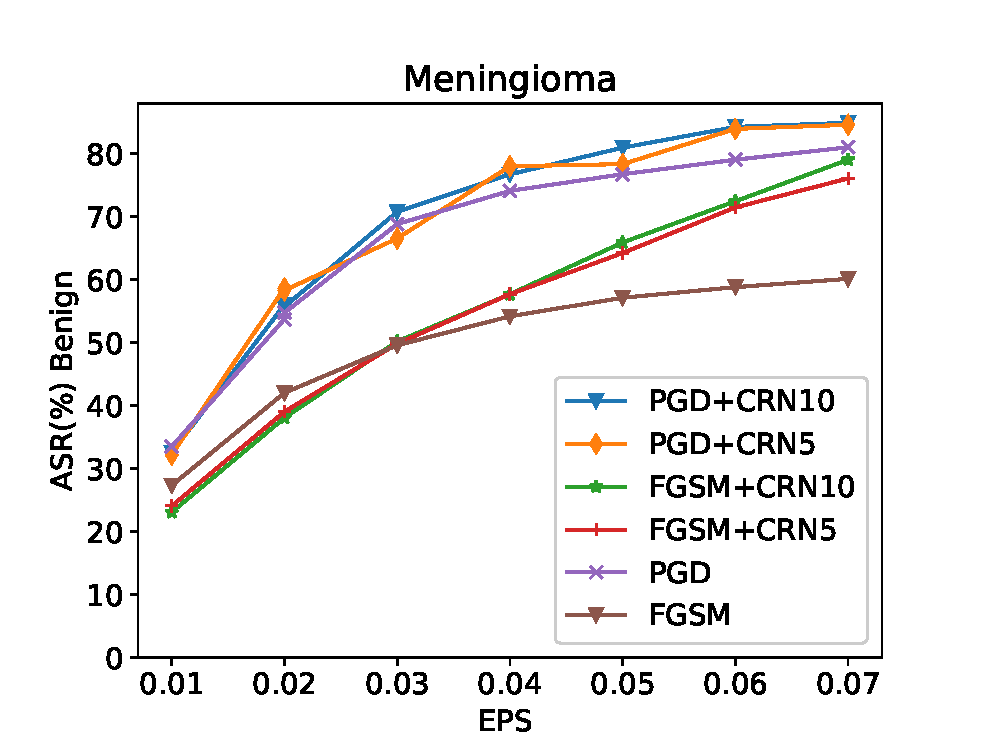
\includegraphics[width=0.32\textwidth]{Meningioma_ASR_EPS.eps}
          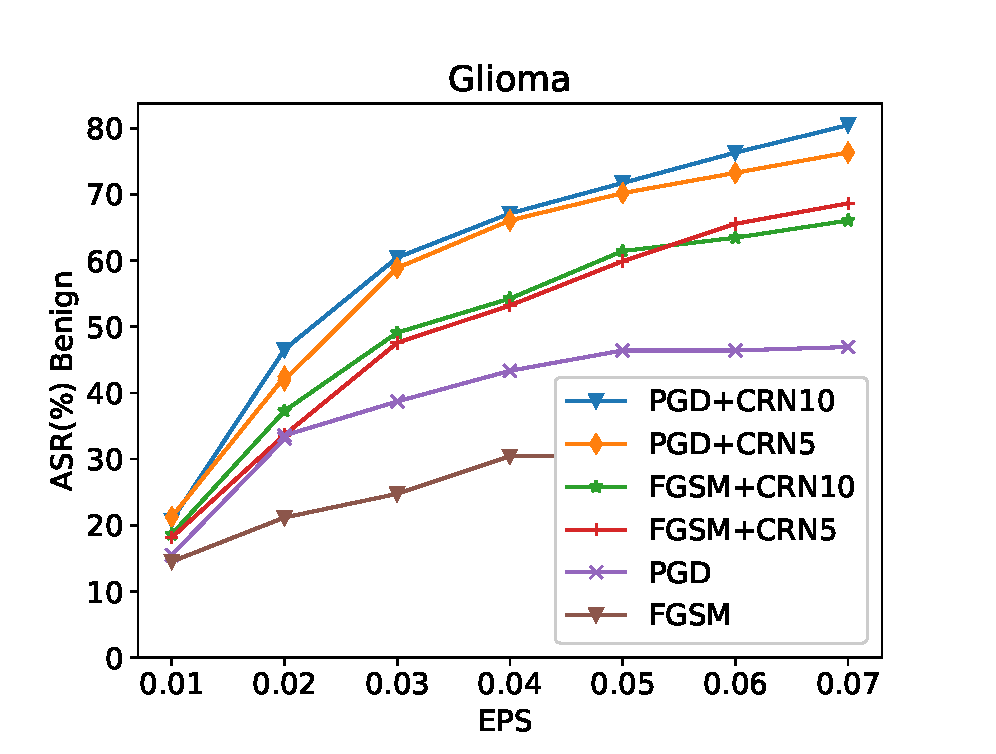
\includegraphics[width=0.32\textwidth]{Glioma_ASR_EPS.eps}
           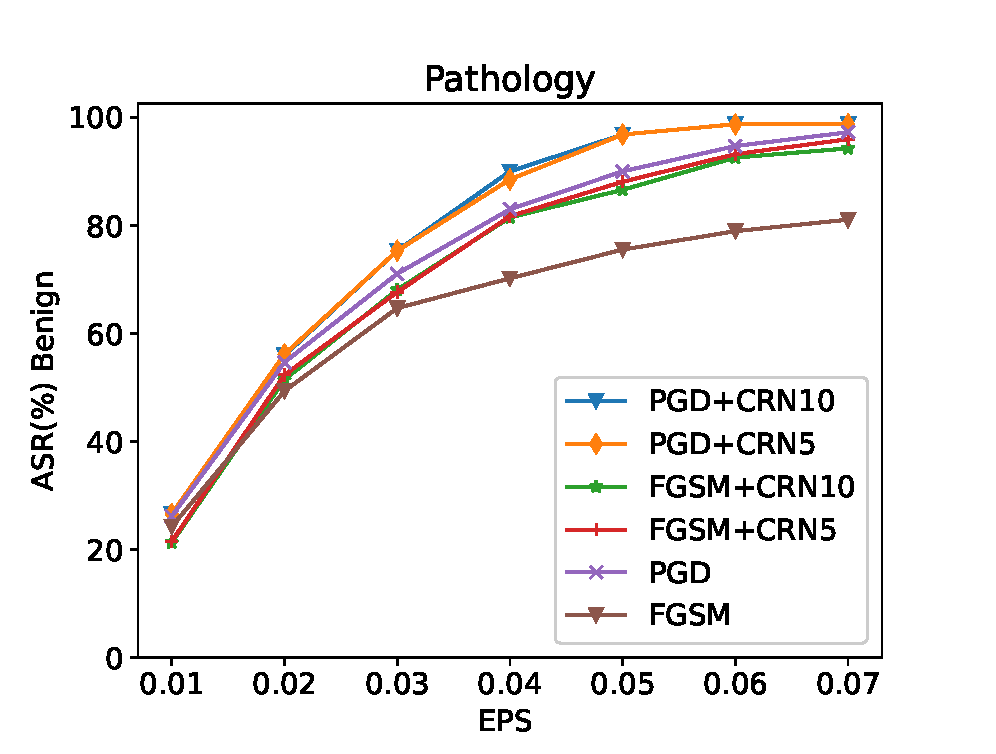
\includegraphics[width=0.32\textwidth]{Pathology_ASR_EPS.eps}
         \caption{Effect of $\epsilon$ on Average ASR on benign clients }
         \label{fig:AASR benign-EPS}
     \end{subfigure}
     \hfill
     \begin{subfigure}
          \centering
         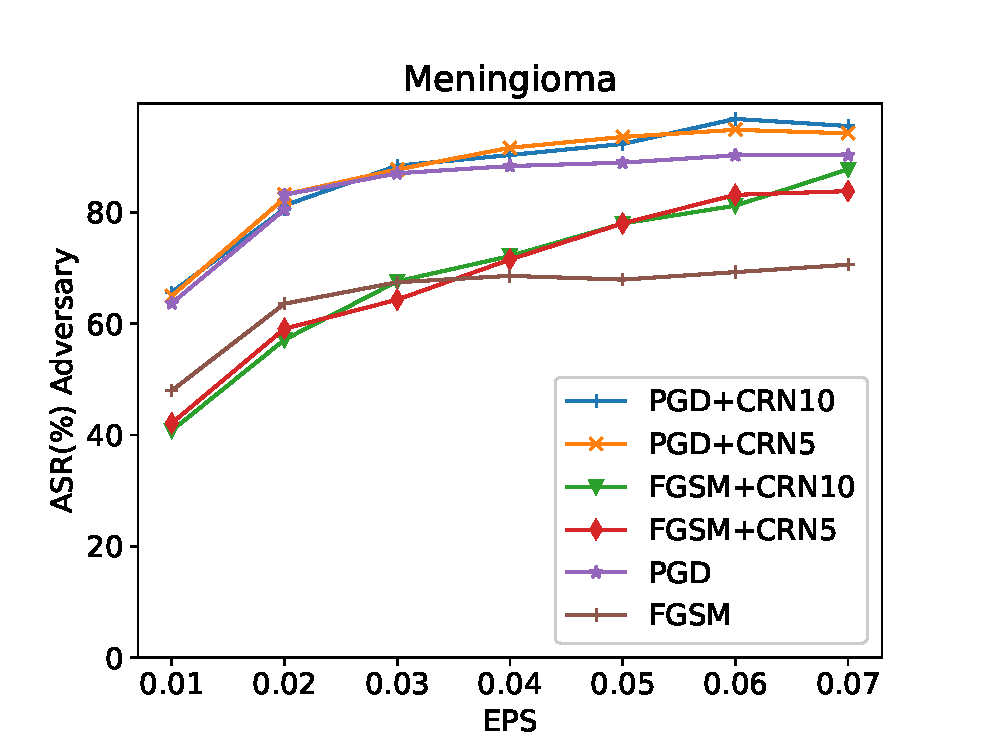
\includegraphics[width=0.32\textwidth]{Meningioma_others_EPS.eps}
          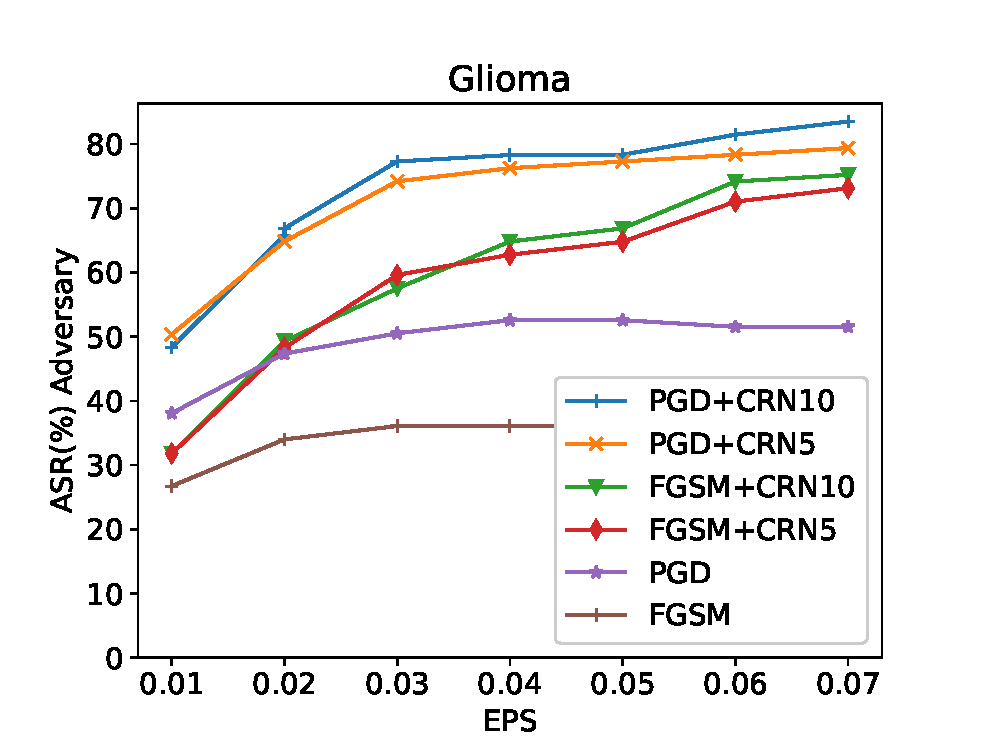
\includegraphics[width=0.32\textwidth]{Glioma_others_EPS.eps}
           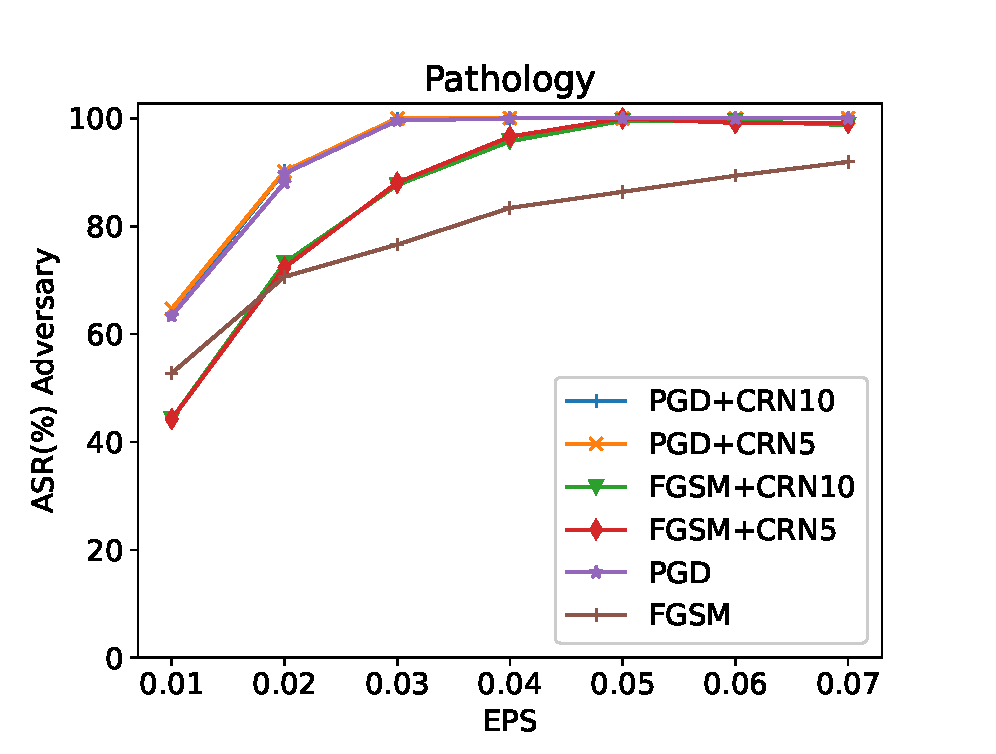
\includegraphics[width=0.32\textwidth]{Pathology_others_EPS.eps}
         \caption{Effect of $\epsilon$ on ASR on the advesarial client }
         \label{fig:AASR malignant-EPS}
     \end{subfigure}
     \hfill
        \caption{Effect of Error perturbation degree $\epsilon$ on attack transferability. FGSM and PGD attack with and without CRN initialization where performed. CRN initalizations used 10 models and another one loading 5.  ASR is calculated on benign and adversary clients. The results of with varying perturbation degrees. The higher ASR on benign clients shows higher transferability}
        \label{fig: epsilon graphs}
\end{figure*}

  Here, we expand the previous findings to the FL settings and discuss whether change in $\epsilon$ can lead to transferability. 
  
We perform three analysis to find important factors in attack success:
\begin{itemize}
    \item We investigate dependency of attacker on $\epsilon$. By visual inspection and ASR evaluation, and as a comparison to previously found optimal known values in centralized  setting.
    \item  We compare  efficiency of models, by discussing their attack preparation time and their ASR.
    \item We also see how attack step $\alpha$ can determine ASR.
\end{itemize}



\section{Results}







% Original images, adversarial images, and corresponding adversarial noise created with FGSM ( ϵ=0.02) in different black-box settings


\subsection{Efficiency analysis}


\begin{figure*}[h!]
     \centering
     \begin{subfigure}
         \centering
         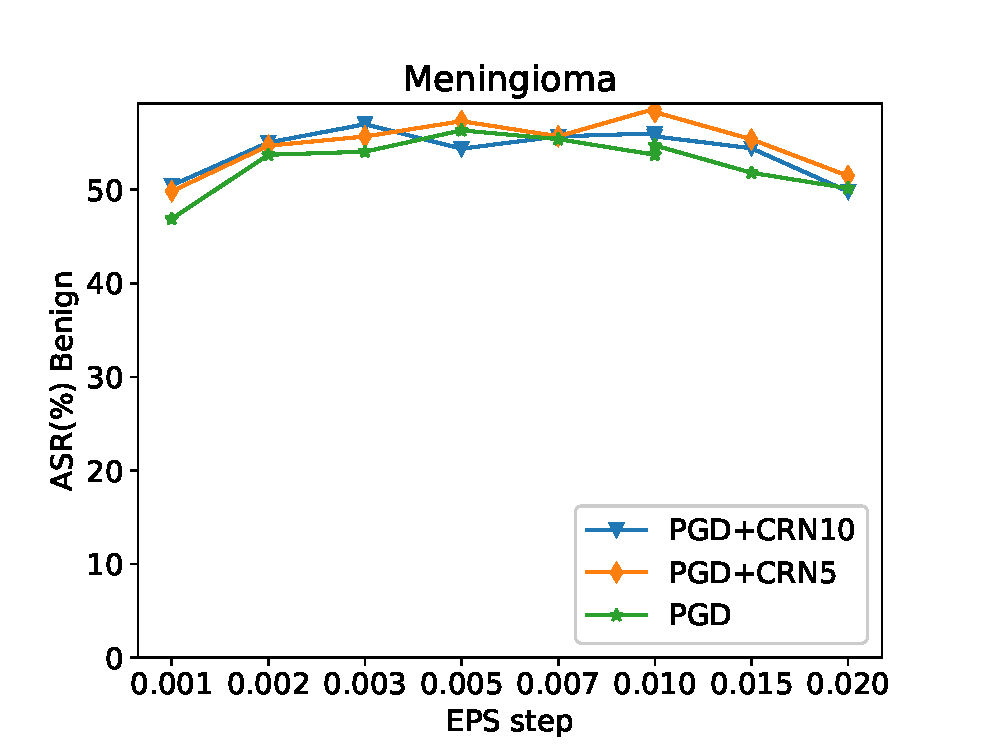
\includegraphics[width=0.32\textwidth]{Meningioma_ASR_EPS_steps.eps}
          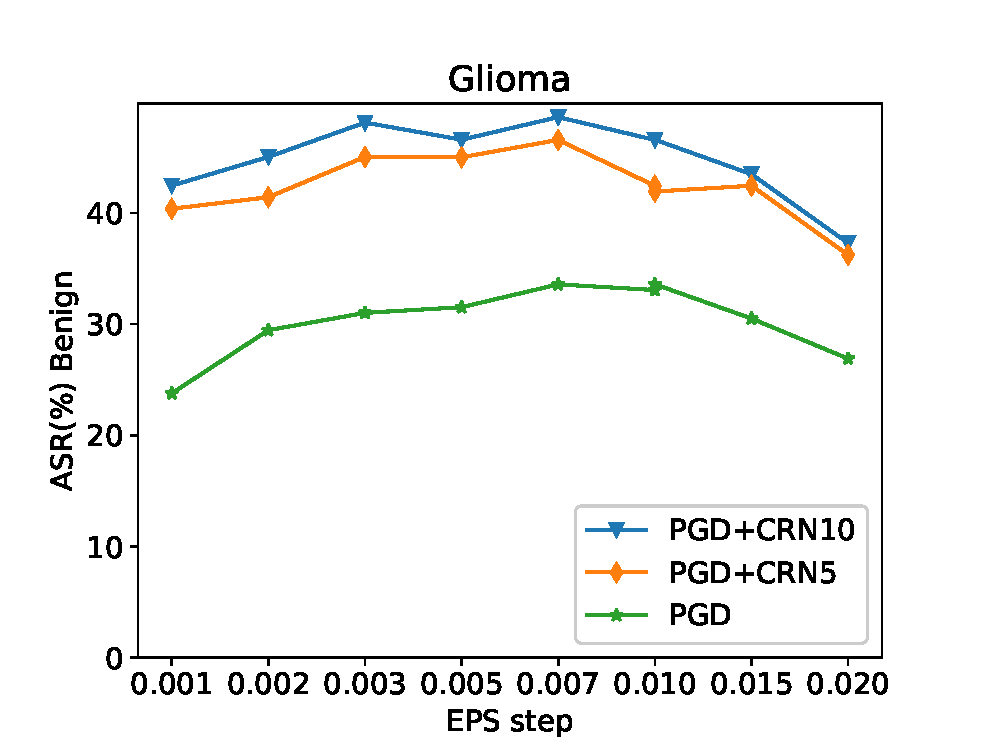
\includegraphics[width=0.32\textwidth]{Glioma_ASR_EPS_steps.eps}
           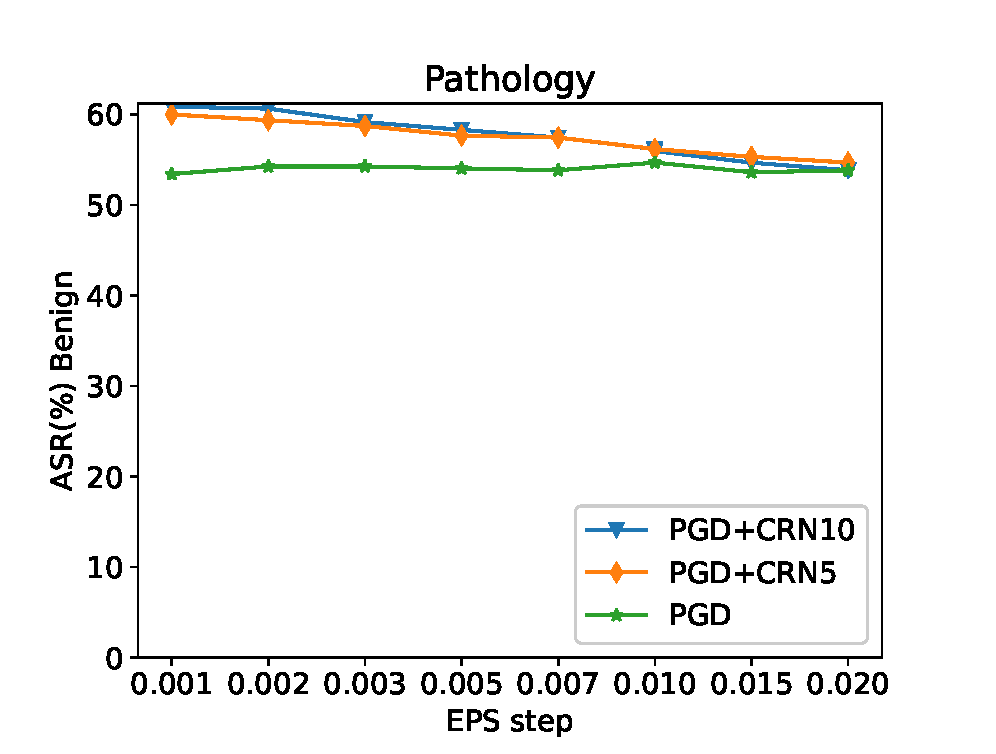
\includegraphics[width=0.32\textwidth]{Pathology_ASR_EPS_steps.eps}
         \caption{Average ASR on benign clients }
         \label{fig:y equals x}
     \end{subfigure}
     \hfill
     \begin{subfigure}
          \centering
         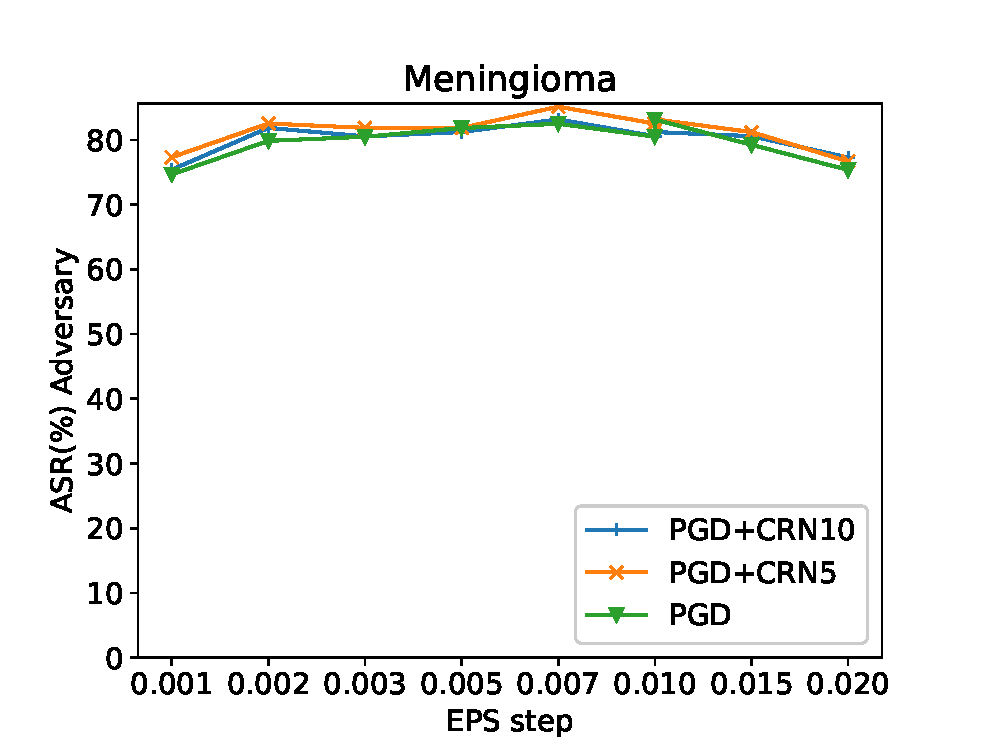
\includegraphics[width=0.32\textwidth]{Meningioma_others_EPS_steps.eps}
          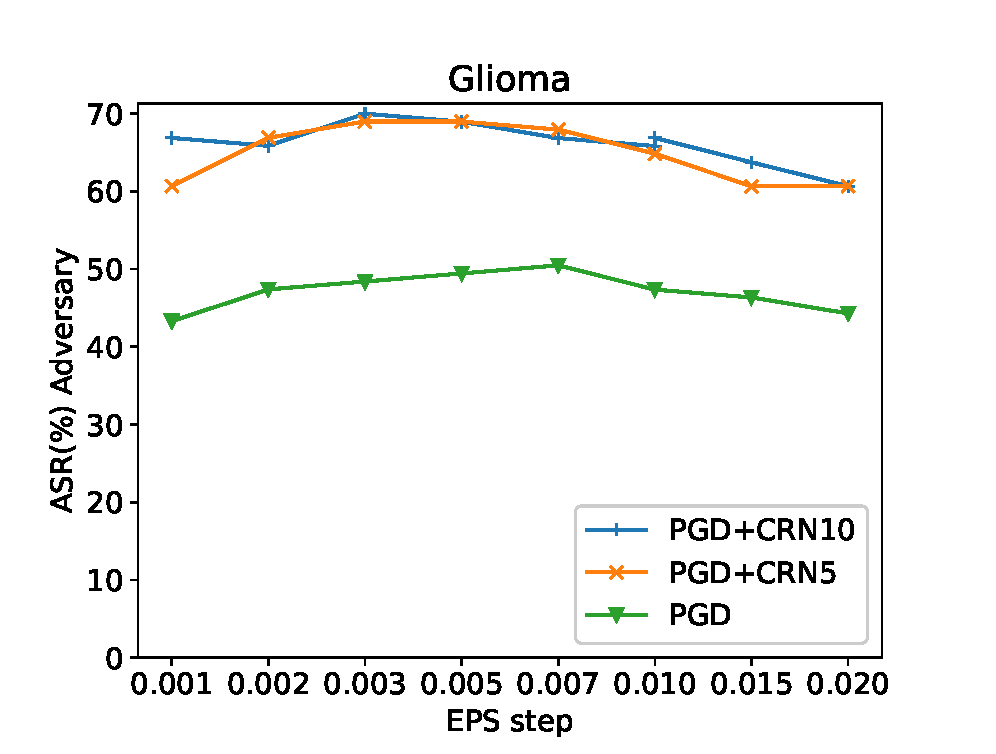
\includegraphics[width=0.32\textwidth]{Glioma_others_EPS_steps.eps}
           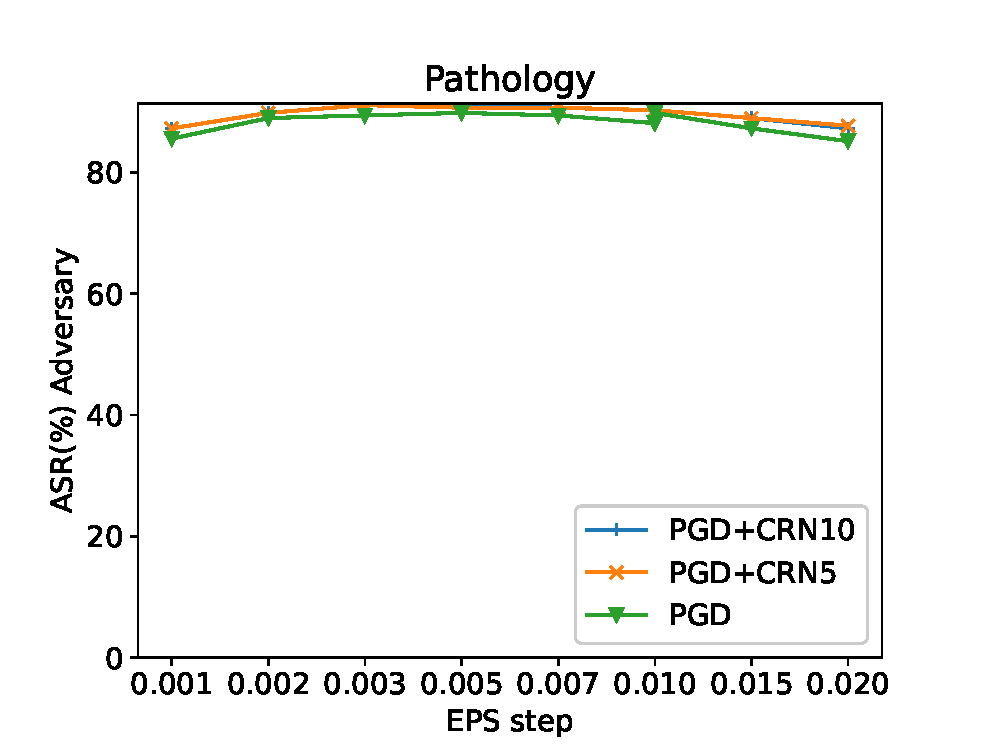
\includegraphics[width=0.32\textwidth]{Pathology_others_EPS_steps.eps}
         \caption{Average ASR on advesarial client }
         \label{fig:y equals x}
     \end{subfigure}
     \hfill
        \caption{Effect of Error perturbation step $\alpha$ on attack transferability. PGD attack with CRN initalizations used 10 models and another one loading 5. ASR is calculated on benign and adversary clients. The results of with varying perturbation steps. The higher ASR on benign clients shows higher transferability}
        \label{fig:three graphs}
\end{figure*}

The models are trained in an FL enviroment. Average test results, or clean accuracy shows the average performance of clients on unperturbed test data. This could be a baseline for comparison of attacks.
Here we compare the computational complexity of iterative algorithms. The comparison is based on the time required to train one batch of adversarial examples, with  $\epsilon=0.05$ and $\alpha=0.001$. The average Attack success rate is the average of ASR for all test samples of all clients and indicates the transferability in the FL network.
As expected \ref{table_time}, the higher iteration rounds take more computation and lead to higher AASR. Generally, computational complexity has a linear dependence on the number of iterations. However, the increase in transferability can vary. If PGD performs poorly initially, having higher iterations doesn't help much. 

Also, CRN does not require additional computation. Similar to single-step methods, computational load is small but increases on high-resolution images. As an example, the pathology dataset requires more calculation than MRI data. 
However, the overall time is far less than iterative models, and also it could enhance the transferability much better. The effect is consistent among different datasets. 
% However,  This means that Pathology images have better AASR than MRI images in baseline and CRN enabled attacks.
% Also,  

% PGD can sometimes perform poorly, even in higher iterations. Enabling the initialization might  


\begin{table}[h!]
\centering
\setlength{\tabcolsep}{6pt}
\renewcommand\arraystretch{1.22}
\caption{ \small Comparison of iterative models and their copmutational efficiency, on performing computations on one batch of data.  ACC shows average client performance for unperturbed test data. AASR is average ASR on all clients.}
\begin{tabular}{| *{5}{c|} }
\hline
Dataset  & Attack type & ACC & AASR & time (sec)
\\   \hline  
\multirow{3}{5em}{Meningioma}     &\textbf{PGD-1+CRN10}&\multirow{3}{3em}{84.12\%}&\textbf{63.92\%} & \textbf{0.217}  \\
 &PGD-20&&27.52\% & 3.423 \\
&PGD-40&&32.99\% & 6.794  \\ \hline
\multirow{3}{4em}{Pathology}     &\textbf{PGD-1+CRN10}&\multirow{3}{3em}{77.01\%}&\textbf{90.92\%} & \textbf{0.354} \\
&PGD-20&&60.98\% & 5.464\\
&PGD-40&&82.27\% & 10.843 \\ \hline
\multirow{3}{3em}{Glioma}     &\textbf{PGD-1+CRN10}&\multirow{3}{3em}{61.84\%}&\textbf{70.55}\% & \textbf{0.216}  \\
&PGD-20&&51.83\% &3.420  \\
&PGD-40&&63.77\% & 6.793  \\ \hline


\end{tabular}
\label{table_time} 
\end{table}




\subsection{Effect perturbation degree}

We performed attack scenarios to evaluate the effect of perturbation degree $\epsilon$  on attack success on the model. We compared the baseline attack to CRN- enabled attacks. ASR is calculated on benign and adversary clients and is shown in Fig \ref{fig: epsilon graphs}.

More successful attacks on adversaries led to higher transferability to benign clients. Low values of $\epsilon$ can decrease transferability to a large extent. $\epsilon$ = 0.01 has poor performance on all the clients. Generally, Higher $\epsilon$ values lead to higher ASR in all scenarios. Although for Meningioma and Glioma images, increasing $\epsilon$ from 0.04 didn't have much positive effect in PGD and FGSM methods on the adversarial client. 
In pathology images, Iterative models can reach perfect accuracy on the adversarial client and have very high transferability.

CRN  has a positive effect on transferability in all scenarios. Also, CRN-enabled models are more dependent on $\epsilon$; their extent can vary depending on the dataset, attack method, and value of $\epsilon$.
Tuning $\epsilon$  might be tricky since performance and imperceptibility should be considered together.High $\epsilon$ values mean more distortion in the image. We performed an FGSM attack with varying $\epsilon$ values to evaluate the perturbation effect visually. Fig \ref{fig:perturbedMRI} shows the results of perturbed images with different perturbation degrees and their comparison with the unperturbed image. Note that perturbation values below  $\epsilon=0.05$ cause limited distortion.


Iterative models can reach high ASR very quickly with increasing $\epsilon$. 

\begin{figure*}[h!]
 \centering
 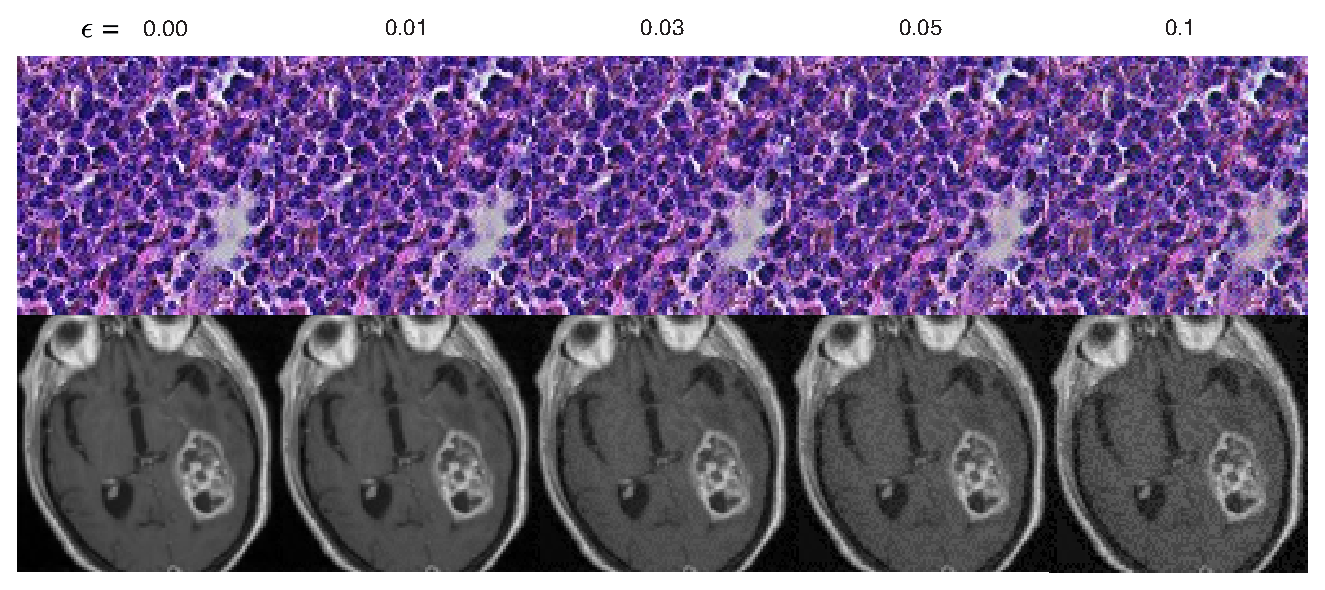
\includegraphics[width=0.8\textwidth]{Adversarial_attacks-5.eps}
 \caption{\small From (a) to (f), normal tumor image, and petrurbed images with FGSM attack, with perturbation parameters: $\epsilon$ = 0.01, 0.03, 0.05,  0.10, respectively}
 \label{fig:perturbedMRI}
\end{figure*}











% \subsection{AATR}
% \begin{table}[h]
% \centering
% \setlength{\tabcolsep}{8pt}
% \renewcommand\arraystretch{1.4}
% \caption{Result of our experiments for PGD attack on Pathology data $\epsilon$ values. The iterative models are trained for 40 rounds with step size of 0.01. \hl{\faQuestion maybe you can change the word for without CRN}}
% % \begin{tabular}{cccccccccccc}
% \begin{tabular}{| *{4}{c|} }\hline
% % Dataset  & Attack type & \multicolumn{2}{c|}{ $\epsilon=0.01$} & \multicolumn{2}{c|}{ $\epsilon=0.03$}           &    \multicolumn{2}{c|}{ $\epsilon=0.05$}    & \multicolumn{2}{c|}{ $\epsilon=0.07$}                                                              \\ \hline
%  Dataset&\multicolumn{3}{c|}{ FGSM}    
% %  &              \multicolumn{3}{c|}{ PGD}                                                                           \\  

%  \cline{2-5}
% &Baseline&CRN5 &CRN10\\\hline

% Meningioma&84.80\%&\textbf{86.31}\%&{84.02\%}
% % \%&83.73\%  &\textbf{84.25}\%  &84.16\%
% \\\hline
% Glioma&82.32\% &87.06\%&\textbf{89.98\%}
% % &74.89\%&\textbf{83.64}\% &82.32\%
% \\\hline

% Pathology&\textbf{90.67\%}&{84.81\%}\%&{85.98\%}
% % \%&79.86\% &86.79\%&\textbf{86.93\%}
% \\\hline



% \end{tabular}
% \label{table_core} 
% \end{table}










\subsection{Effect perturbation step}


Another critical parameter is the step of change in iterative methods. {$\alpha$} is shown to be highly deterministic in specific settings, but is not yet investigated in MIA domain. To evaluate how $\alpha$ can affect transferability, we examined the clients with $\eps=0.03$. Under various steps. The general observation is that there is an optimal middle range the same as $\epsilon$. The step size of 0.007 led to the highest transferability in MRI images. Larger steps led to a sharp decrease in transferability. For pathology images, midspans, about 0.007 led to the best ASR on the adversary, and higher values decreased both ASR on adversary and transferability. However, smaller steps also had high ASR values. 







\subsection{Error tranferability}




Another measure is the average error transfer rate (AETR). Although PGD outperforms FGSM in ASR, in AETR, the results are close. PGD is trained for 40 iterations, and the models are compared with and without CRN.
Both FGSM and PGD having high AETR suggest that although FGSM might not be able to produce high-quality samples in general, the good examples which can fool the adversary are also highly transferable to benign clients. And can be better than PGD samples. CRN generally increases the AETR. 




\begin{table*}[h!]
\centering
\setlength{\tabcolsep}{8pt}
\renewcommand\arraystretch{1.4}
\caption{Result of Average Error Transfer Rate (AETR) for FGSM and PGD methods, with and without CRN initalization }
% \begin{tabular}{cccccccccccc}
\begin{tabular}{| *{7}{c|} }\hline
% Dataset  & Attack type & \multicolumn{2}{c|}{ $\epsilon=0.01$} & \multicolumn{2}{c|}{ $\epsilon=0.03$}           &    \multicolumn{2}{c|}{ $\epsilon=0.05$}    & \multicolumn{2}{c|}{ $\epsilon=0.07$}                                                              \\ \hline
 Dataset&\multicolumn{3}{c|}{ FGSM}     &              \multicolumn{3}{c|}{ PGD}                                                                           \\  

 \cline{2-7}
&Baseline&CRN5 &CRN10&Baeline&CRN5&CRN10\\\hline

Meningioma&84.80\%&\textbf{86.31}\%&{84.02}\%&83.73\%  &\textbf{84.25}\%  &84.16\%\\\hline
Glioma&82.32\% &87.06&\textbf{89.98}&74.89\%&\textbf{83.64}\% &82.32\%\\\hline

Pathology&\textbf{90.67\%}&{84.81}\%&{85.98}\%&79.86\% &86.79\%&\textbf{86.93\%}\\\hline



\end{tabular}
\label{table_core} 
\end{table*}


% \newpage



\section{Discussion}

Our results admit the prior research about vulnerability of FL networks
\cite{goldblum2020dataset,liu2022threats,sun2019can,fang2020local,wang2020attack,song2020analyzing,wilkinson2016fair,van2022ai,miotto2016deep,costa2021covert,bouacida2021vulnerabilities} and MI systems 
 \cite{ma2021understanding,finlayson2019adversarial,gupta2022vulnerability,bortsova2021adversarial}  to adversaraial attacks.

% Our results suggest that even in a DP-enabled setting, adversarial samples generated on one client can be highly transferable.

We also found that differential privacy might have partial effect on attacker's success. In fact, DP caused the lower ASR in surrogate than the adversary clients.
% But it can not be considered as an effective counter-measure.
Although some research support DP, our findings suggest that more with ones who describe it as an option but not very reliable. \cite{bouacida2021vulnerabilities}. Also, the accuracy compromise coming with noise should be considered. \cite{canonne2020discrete} \cite{wang2019privacy}.
\\In our experiments the attacker did not tamper with the training procedure. his is unlike backdoor or poisoning attacks.\cite{lyu2020privacy}\cite{lyu2020threats}. where the attacker performs malicious activities during training, and opens the way for detection methods.
Also, CRN initialization led to faster attacks with higher transferability. This section discusses our findings, how they could be important in the MI domain, and what to consider when setting up FL MI infrastructure.



\subsection{Transferability}
% The practice could be that not always adding noise is better, especially in medical images where compromising accuracy affects patients. Other methods have their problems as stated before, \cite{yin2022adc,yuan2019adversarial,uesato2018adversarial} mainly compromising performance or working in certain conditions. 
% Further research might consider defense models of FL networks. 
Our experiments aimed to asses some factors in transferability. However, other than investigated factors, we found three other parameters might highly predict transferability.

\textbf{Benign/Adversary correlation:} Our results show that ASR on benign and adversary clients are highly correlated. Hence, for the adversary to ensure it can fool other clients in a black-box setting, it needs to obtain good results on its own data and model. So tuning the hyperparamets, data preprocessing can be all effective as long as they improve ASR on adversary.

\textbf{AETR/ASR difference:}, Attacks have higher AETR than ASR, which enables the adversary to subsample examples to achieve higher transferability. 
%. In black-box models, the attack results might vary from low transferability to similar to white-box. Depending on many parameters. But when implementing in a
% FL environment, the results are closer to the white-box setting. 
% This finding admits that models trained in FL setting keep their traditional ML vulnerabilities, and FL imposes an additional threat. Leading to aggregated vulnerabilty.\hl{  \faClockOshayad ye graph peyda Koni ke ASR ro ba white/black tozih bede}

\textbf{Attack domain}: We observed that transferability is specific within imaging domains, which is consistent with prior findings.\cite{bortsova2021adversarial} Attacks on Pathology images were consistently more successful than MRI images. 

% \subsection{Effect of parameters}
\textbf{Perturbation parameter}
% $\epsilon$  As shown in \ref{fig: epsilon graphs} 
Level of $\epsilon$ can substantially change transferability. Increasing $\epsilon$ does not improve ASR from a certain point, but adding CRN can increase the dependency. The best perturbation range in our experiments is around 0.03-0.05. These results suggest that conclusions in a centralized setting might not apply to an FL environment. And it shows different transferability behavior or parameter dependence.

\textbf{Step parameter } Our findings show that common $\alpha$ values have a  negligible effect on the final results, aside from too small or too large values. The reason could be that $\alpha$ similar to  $\epsilon$  bounds the change in each iteration, but generally, its values are one order of magnitude less than $\epsilon$. 


\subsection{Efficiency}
% Attacks can substantially differ in the computational requirements, 
% which can have practical implications in the MIA domain.
Our results show that initialization can be influential in computational efficiency. PGD with random intialization requires high computational power wihch migh be burdensome for High-resolution or large-batch training. Using CRN leads to much fewer computational requirements. Single-step attacks can be $20 \sim 30 \times$ less expensive than iterative models with 40 iterations and higher ASR. 
More minor GPU requirements \\Adversaries might be capable of attacks using high-volumes of data or with multiple devices by using CRN.
\\Standard ways of simulating attacks, like adaptive models and sanity checks, \cite{carlini2019evaluating} might be unfeasible in their traditional way. An adversary might have more knowledge than what is assumed in evaluation models, hence using more efficient methods or attacks with unexpected devices.



\subsection{Practical implications and suggestions}

In the following paragraphs, we discuss the motivations that cause adversarial attacks .

The large healthcare economy causes more benefit for malicious behavior, as there are existing reports of pervasive fraud in healthcare. Medical record manipulation for financial purposes \cite{ma2021understanding} fake trial reports\cite{george2015data} in radiology \cite{chowdhry2014image} and pathology\cite{suvarna2001histopathology} are widespread practices, and already made billions of dollars profit \cite{graese2016assessing} for fraudsters. Also, advanced fabrication algorithms and hard to detect methods are always intruguing for fradusters. Existing Manipulations like altering the visual features of images, or using photo editing software, \cite{chowdhry2014image} can result in images of benign subjects classified as malignant.\cite{xia2020pseudo}
\cite{sun2020adversarial}, but with visual distoration. In contrast, adversarial attacks are imperceptible, do not require manual intervention, and have high transferability. That gives a significant incentive for potential fraudsters to utilize adversarial attacks for high potential revenue. \\For example, consider a hypothetical case in which insurance companies utilize AI-based systems to approve a disease and get refund. A malicious person could add adversarial noise to images to manipulate insurance companies. Or consider if a person tries to bill insurance companies by reporting falsified surgical procedures. They can use attack algorithms to synthesize fake MRI and send it to the target company.
\\These vulnerabilities have some implications for clinical decision-makers, stakeholders, and insurance companies, who consider deploying FL or AI pipelines , which will be discussed in the following.
 
\begin{enumerate}[(i)]
    \item  First, they might take the pervasive motivation of manipulation and fraud into consideration, and beware of the financial and incentive \cite{finlayson2019adversarial}
    \item Second, having secure infrastructure in training phase does not guarantee safety in the deployment phase. So they might distinguish between these two, and consider redundant ways of incorporating AI in their MIA pipelines.
\item  Third, they might reconsider size and level of trust in collaborative/FL networks. Smaller networks with trusted parties have lower probability of having potential adversary.
\item Fourth, by not enforcing same data pre-processing pipelines, they might be able to hinder the adversary. They might also consider that having disparate data affects performance or even convergence of FL network.\cite{li2019convergence}. and how should they deal with the compromise between safety and performance.
\end{enumerate}

\\For developers of MIA systems these findings can have consider four things :

\begin{enumerate}[(i)]
    \item They can help end-users and clinicians by providing them more information other than model outputs. For example, adding explainable system reports helps the clinicians evaluate the legitimacy of predictions.
    \item Standard ways of evaluating robustness \cite{carlini2019evaluating}are not recommended in FL setting. so they might consider scenarios where adversary traces the global model, and has more knowledge, or attacks with unexpected devices.
    \item There is no universal factors to predict the capability of adversary, so they might consider existing research to important factor for each setting, or they might to a brute-force search to find upper-bounds of vulnerability. \cite{carlini2019evaluating} 
     \item Despite not having a universal defense method, there are limited case-specific defense models shown to work on some datasets, \cite{graese2016assessing} so developers might consider looking into potnetial defense method for their usecase.
\end{enumerate}





% One implication it might give is that, we might increase the robustness of FL network, 


\section{Conclusion}


This paper investigated adversarial attacks on federated MIA systems and discussed the crucial parameters on their transferability. We also proposed a new method that leverages the federated setting to improve the attack success rate and reduce the computation burden.
We saw that tuning the parameters can substantially improve transferability.
We also observed that adequately using noise from previous model updates can effectively improve computational load and has the potential to be well integrated into the existing attack methods.

Future lines of research could be to improve existing defense methods,\cite{sun2019can,wang2020attack,shao2019stochastic,li2019distributed,ma2019privacy,li2020multi ,yin2022adc,zheng2020efficient,yuan2019adversarial,uesato2018adversarial} , towards a universal defense algorithm. Another line of research could be how to utilize distributed nature of FL networks to protect all participating clients, or if collaboration can be used to enhance the current defense methods.\\
We hope this research could benefit healthcare institutions and hospitals considering bringing in AI or joining FL networks to be warier of the threat of adversarial examples. For medical institutions and managers of hospitals and insurance companies, this research might show that they might pay extra attention to the AI pipelines and FL deployments. This research might help security experts reconsider standard vulnerability analysis and consider different scenarios where a capable adversary proposes fast and efficient attacks. For ML researchers involved in bringing in FL networks, a line of research can devise more reliable defense methods.


% \begin{equation}\label{diode_voltage_waveform_B}
%     v(\theta) = V_{DC} + V(f_0)\sin(\theta)
% \end{equation}
% where $V(f_0)$ is the fundamental frequency component of the voltage across the rectifying element, $V_{DC}$ is the DC component, $V_{DC} = V(f_0)$ and $\theta = 2\pi f_0 t$. The current waveform contains infinite frequency components, and can be written as

% \begin{equation}\label{diode_current_waveform_time_domain}
%     i(\theta) = 2\pi I_{DC}\delta\left(\theta-\frac{3\pi}{2} - 2n\pi\right), \hskip 1pc n = 0,1,...,\infty
% \end{equation}


% \begin{equation}\label{diode_current_waveform_finv}
% i(\theta) =
% \begin{cases}
%     0, & 0 \leq \theta < \pi\\
%     2I_{DC}, & \pi \leq \theta < 2\pi
% \end{cases}
% \end{equation}


% \begin{equation}\label{eff_finv}
%     \eta = \frac{P_{DC}}{P(f_0)} = \frac{2V_{DC}I_{DC}}{V(f_0)I(f_0)} = \frac{2\frac{2}{\pi}V(f_0)\frac{\pi}{4}I(f_0)}{V(f_0)I(f_0)} = 1
% \end{equation}

 
%  \caption{RF-DC conversion efficiency versus DC load fixed available input powers with 0.6\,dB matching network loss de-embedded.  The maximum efficiency of 72.8\% occurred at 8\,dBm with $R_{DC}$ = 742\,$\Omega$, which is lower than the 1080\,$\Omega$ found during source-pull.  However, the efficiency at 1080\,$\Omega$ is 69.9\% which is very close to the peak value.}\label{final_dc_sweep}





% \begin{figure}[ht!]
% \centering
% \includegraphics[width=3.5in]{pdf/10.pdf}
% \caption{Time-domain non-linear rectifier measurement block diagram. The SWAP \cite{SWAP} performs sampling of current and voltage and the calibration refers the sampled quantities to the reference planes at the DUT. The drain output DC resistance $R_{DC}$ , the gate bias $V_{GS}$ and the gate RF impedance $Z_g$ are varied as the input power at the drain is swept from 10 to 42\,dBm.}
% \label{measurement_setup}
% \end{figure}


% \section*{Acknowledgment}


%Dr. Reveryrand would like to acknowledge the funding by XLIM, Limoges, France. 
% The authors would like to thank Dr. Chaoning Zhang.


% if have a single appendix:
%\appendix[Proof of the Zonklar Equations]
% or
%\appendix  % for no appendix heading
% do not use \section anymore after \appendix, only \section*
% is possibly needed

% use appendices with more than one appendix
% then use \section to start each appendix
% you must declare a \section before using any
% \subsection or using \label (\appendices by itself
% starts a section numbered zero.)
%

% ============================================
%\appendices
%\section{Proof of the First Zonklar Equation}
%Appendix one text goes here %\cite{Roberg2010}.

% you can choose not to have a title for an appendix
% if you want by leaving the argument blank
%\section{}
%Appendix two text goes here.


% use section* for acknowledgement
%\section*{Acknowledgment}


%The authors would like to thank D. Root for the loan of the SWAP. The SWAP that can ONLY be usefull in Boulder...


% Can use something like this to put references on a page
% by themselves when using endfloat and the captionsoff option.
\ifCLASSOPTIONcaptionsoff
  \newpage
\fi



% trigger a \newpage just before the given reference
% number - used to balance the columns on the last page
% adjust value as needed - may need to be readjusted if
% the document is modified later
%\IEEEtriggeratref{8}
% The "triggered" command can be changed if desired:
%\IEEEtriggercmd{\enlargethispage{-5in}}

% ====== REFERENCE SECTION

% \begin{thebibliography}{1}

% IEEEabrv,
% \bibliography{IEEE_references}  %%% Uncomment this line and comment out the ``thebibliography'' section below to use the external .bib file (using bibtex) .

\printbibliography
% \bibliographystyle{IEEEtran}
% \bibliography{IEEEabrv}

% \bibliographystyle{IEEEtran}
% \bibliography{IEEEabrv,Bibliography}
% \end{thebibliography}
% % biography section
% 
% If you have an EPS/PDF photo (graphicx package needed) extra braces are
% needed around the contents of the optional argument to biography to prevent
% the LaTeX parser from getting confused when it sees the complicated
% \includegraphics command within an optional argument. (You could create
% your own custom macro containing the \includegraphics command to make things
% simpler here.)
%\begin{biography}[{\includegraphics[width=1in,height=1.25in,clip,keepaspectratio]{mshell}}]{Michael Shell}
% or if you just want to reserve a space for a photo:

% ==== SWITCH OFF the BIO for submission
% ==== SWITCH OFF the BIO for submission
% \begin{IEEEbiography}[{\includegraphics[width=1in,height=1.25in,clip,keepaspectratio]{photo/mike.png}}]{Michael Roberg}
% (S'09) received the B.S.E.E degree from Bucknell University, Lewisburg, PA, in 2003, the M.S.E.E. degree from the University of Pennsylvania, Philadelphia, in 2006, and the Ph.D. degree from the University of Colorado at Boulder in 2012. From 2003 to 2009, he was an Engineer with Lockheed Martin–MS2, Moorestown, NJ, where he was involved with advanced phased-array radar systems. His current research interests include high efficiency microwave PA theory and design, microwave power rectifiers, MMIC design, and high-efficiency radar and communication system transmitters. He is currently employed by TriQuint Semiconductor - Defense Products and Foundry Services in Richardson, TX working on wideband high efficiency GaN MMIC PA design.
% \end{IEEEbiography}

%% if you will not have a photo at all:
%\begin{IEEEbiographynophoto}{Ignacio Ramos}
%(S'12) received the B.S. degree in electrical engineering from the University of Illinois at Chicago in 2009, and is currently working toward the Ph.D. degree at the University of Colorado at Boulder. From 2009 to 2011, he was with the Power and Electronic Systems Department at Raytheon IDS, Sudbury, MA. His research interests include high-efficiency microwave power amplifiers, microwave DC/DC converters, radar systems, and wireless power transmission.
%\end{IEEEbiographynophoto}

%% insert where needed to balance the two columns on the last page with
%% biographies
%%\newpage

%\begin{IEEEbiographynophoto}{Jane Doe}
%Biography text here.
%\end{IEEEbiographynophoto}
% ==== SWITCH OFF the BIO for submission
% ==== SWITCH OFF the BIO for submission



% You can push biographies down or up by placing
% a \vfill before or after them. The appropriate
% use of \vfill depends on what kind of text is
% on the last page and whether or not the columns
% are being equalized.

\vfill

% Can be used to pull up biographies so that the bottom of the last one
% is flush with the other column.
%\enlargethispage{-5in}


% \section{To do list}
% \subsection{Quick things}

% \begin{itemize}
% \item evaluate iid-ness and see if your data was non-iid and mention it
% \end{itemize}
% \subsection{Absolutely necessary}
% %   \item add pathology image to figure perturbation of MRI
% \subsubsection{Paper}
% \begin{itemize}
%     % \item paraphrise + shorten FL and DP sections
%     % \item baad yebar ba dide Chaoning bekhun
% \end{itemize}
% \subsubsection{Coding}
% \begin{itemize}

% \end{itemize}
% \subsection{Maybe later}
% \subsubsection{coding}
% \begin{itemize}
%   \item mituni regularization ro aksesho bekeshi
%  \item SSIM/PSNR
% graph?
%     \item mituni correlation begiri beine ASR advresary o benign
%     \item mituni  baraye GC neshun bedi ke l2 norm payeen tar miad (mesle khode. maqale asli) pas in raveshe ma natije dade va GC kare khubi bude
%     \item gradient alignment? bara in yeki umade mige gradient alignment kheili moheme\cite{https://www.usenix.org/system/files/sec19-demontis.pdf}
%     \item Maybe you can discuss the saliency attention maps in different clients/ and show they are the same. Tell even DP can not distract the models to where they should focus
  
%   \item Maybe doing gradcam? 
%     \item  Do the graphs of eps step with eps= 0.03 to have similar with others, AATR is not changeable from eps=0.03
%       \item effect of loaded models on performance?
  
%     \item make code readable/extendable?
   
%     \item Maybe fix for Chest and Tumors?
%     \item time table with other EPS? NOoo
%     \item find a way to show that the networks are very different under DP (maybe by visualization)
% \end{itemize}

% \subsubsection{Paper}
% \begin{itemize}
%     \item 
% \\\hl{\faClockO }

%     \item maybe adding detailed graph for each participant as an Appendix?
% \end{itemize}


% \bibliographystyle{unsrtnat}
% \bibliography{dissertation} 
% I hope this helps you get started!
% Moritz
